\documentclass[twoside]{book}

% Packages required by doxygen
\usepackage{fixltx2e}
\usepackage{calc}
\usepackage{doxygen}
\usepackage[export]{adjustbox} % also loads graphicx
\usepackage{graphicx}
\usepackage[utf8]{inputenc}
\usepackage{makeidx}
\usepackage{multicol}
\usepackage{multirow}
\PassOptionsToPackage{warn}{textcomp}
\usepackage{textcomp}
\usepackage[nointegrals]{wasysym}
\usepackage[table]{xcolor}

% Font selection
\usepackage[T1]{fontenc}
\usepackage[scaled=.90]{helvet}
\usepackage{courier}
\usepackage{amssymb}
\usepackage{sectsty}
\renewcommand{\familydefault}{\sfdefault}
\allsectionsfont{%
  \fontseries{bc}\selectfont%
  \color{darkgray}%
}
\renewcommand{\DoxyLabelFont}{%
  \fontseries{bc}\selectfont%
  \color{darkgray}%
}
\newcommand{\+}{\discretionary{\mbox{\scriptsize$\hookleftarrow$}}{}{}}

% Page & text layout
\usepackage{geometry}
\geometry{%
  a4paper,%
  top=2.5cm,%
  bottom=2.5cm,%
  left=2.5cm,%
  right=2.5cm%
}
\tolerance=750
\hfuzz=15pt
\hbadness=750
\setlength{\emergencystretch}{15pt}
\setlength{\parindent}{0cm}
\setlength{\parskip}{0.2cm}
\makeatletter
\renewcommand{\paragraph}{%
  \@startsection{paragraph}{4}{0ex}{-1.0ex}{1.0ex}{%
    \normalfont\normalsize\bfseries\SS@parafont%
  }%
}
\renewcommand{\subparagraph}{%
  \@startsection{subparagraph}{5}{0ex}{-1.0ex}{1.0ex}{%
    \normalfont\normalsize\bfseries\SS@subparafont%
  }%
}
\makeatother

% Headers & footers
\usepackage{fancyhdr}
\pagestyle{fancyplain}
\fancyhead[LE]{\fancyplain{}{\bfseries\thepage}}
\fancyhead[CE]{\fancyplain{}{}}
\fancyhead[RE]{\fancyplain{}{\bfseries\leftmark}}
\fancyhead[LO]{\fancyplain{}{\bfseries\rightmark}}
\fancyhead[CO]{\fancyplain{}{}}
\fancyhead[RO]{\fancyplain{}{\bfseries\thepage}}
\fancyfoot[LE]{\fancyplain{}{}}
\fancyfoot[CE]{\fancyplain{}{}}
\fancyfoot[RE]{\fancyplain{}{\bfseries\scriptsize Generated on Wed Oct 11 2017 16\+:11\+:57 for Figura by Doxygen }}
\fancyfoot[LO]{\fancyplain{}{\bfseries\scriptsize Generated on Wed Oct 11 2017 16\+:11\+:57 for Figura by Doxygen }}
\fancyfoot[CO]{\fancyplain{}{}}
\fancyfoot[RO]{\fancyplain{}{}}
\renewcommand{\footrulewidth}{0.4pt}
\renewcommand{\chaptermark}[1]{%
  \markboth{#1}{}%
}
\renewcommand{\sectionmark}[1]{%
  \markright{\thesection\ #1}%
}

% Indices & bibliography
\usepackage{natbib}
\usepackage[titles]{tocloft}
\setcounter{tocdepth}{3}
\setcounter{secnumdepth}{5}
\makeindex

% Hyperlinks (required, but should be loaded last)
\usepackage{ifpdf}
\ifpdf
  \usepackage[pdftex,pagebackref=true]{hyperref}
\else
  \usepackage[ps2pdf,pagebackref=true]{hyperref}
\fi
\hypersetup{%
  colorlinks=true,%
  linkcolor=blue,%
  citecolor=blue,%
  unicode%
}

% Custom commands
\newcommand{\clearemptydoublepage}{%
  \newpage{\pagestyle{empty}\cleardoublepage}%
}


%===== C O N T E N T S =====

\begin{document}

% Titlepage & ToC
\hypersetup{pageanchor=false,
             bookmarks=true,
             bookmarksnumbered=true,
             pdfencoding=unicode
            }
\pagenumbering{roman}
\begin{titlepage}
\vspace*{7cm}
\begin{center}%
{\Large Figura }\\
\vspace*{1cm}
{\large Generated by Doxygen 1.8.9}\\
\vspace*{0.5cm}
{\small Wed Oct 11 2017 16:11:57}\\
\end{center}
\end{titlepage}
\clearemptydoublepage
\tableofcontents
\clearemptydoublepage
\pagenumbering{arabic}
\hypersetup{pageanchor=true}

%--- Begin generated contents ---
\chapter{Namespace Index}
\section{Packages}
Here are the packages with brief descriptions (if available)\+:\begin{DoxyCompactList}
\item\contentsline{section}{\hyperlink{namespace_calcular_area_y_perimetro}{Calcular\+Area\+Y\+Perimetro} }{\pageref{namespace_calcular_area_y_perimetro}}{}
\item\contentsline{section}{\hyperlink{namespace_calcular_perimetro_y_area}{Calcular\+Perimetro\+Y\+Area} }{\pageref{namespace_calcular_perimetro_y_area}}{}
\item\contentsline{section}{\hyperlink{namespace_calcular_perimetro_y_area_1_1_properties}{Calcular\+Perimetro\+Y\+Area.\+Properties} }{\pageref{namespace_calcular_perimetro_y_area_1_1_properties}}{}
\end{DoxyCompactList}

\chapter{Hierarchical Index}
\section{Class Hierarchy}
This inheritance list is sorted roughly, but not completely, alphabetically\+:\begin{DoxyCompactList}
\item \contentsline{section}{Calcular\+Area\+Y\+Perimetro.\+Figura}{\pageref{class_calcular_area_y_perimetro_1_1_figura}}{}
\begin{DoxyCompactList}
\item \contentsline{section}{Calcular\+Area\+Y\+Perimetro.\+Círculo}{\pageref{class_calcular_area_y_perimetro_1_1_c_xC3_xADrculo}}{}
\item \contentsline{section}{Calcular\+Area\+Y\+Perimetro.\+Rectángulo}{\pageref{class_calcular_area_y_perimetro_1_1_rect_xC3_xA1ngulo}}{}
\item \contentsline{section}{Calcular\+Area\+Y\+Perimetro.\+Triángulo}{\pageref{class_calcular_area_y_perimetro_1_1_tri_xC3_xA1ngulo}}{}
\end{DoxyCompactList}
\item Form\begin{DoxyCompactList}
\item \contentsline{section}{Calcular\+Perimetro\+Y\+Area.\+Form1}{\pageref{class_calcular_perimetro_y_area_1_1_form1}}{}
\item \contentsline{section}{Calcular\+Perimetro\+Y\+Area.\+Form2}{\pageref{class_calcular_perimetro_y_area_1_1_form2}}{}
\item \contentsline{section}{Calcular\+Perimetro\+Y\+Area.\+Form3}{\pageref{class_calcular_perimetro_y_area_1_1_form3}}{}
\item \contentsline{section}{Calcular\+Perimetro\+Y\+Area.\+form\+Principal}{\pageref{class_calcular_perimetro_y_area_1_1form_principal}}{}
\end{DoxyCompactList}
\end{DoxyCompactList}

\chapter{Class Index}
\section{Class List}
Here are the classes, structs, unions and interfaces with brief descriptions\+:\begin{DoxyCompactList}
\item\contentsline{section}{\hyperlink{class_calcular_area_y_perimetro_1_1_c_xC3_xADrculo}{Calcular\+Area\+Y\+Perimetro.\+Círculo} \\*Clase \hyperlink{class_calcular_area_y_perimetro_1_1_c_xC3_xADrculo}{Círculo} que hereda de la Clase \hyperlink{class_calcular_area_y_perimetro_1_1_figura}{Figura}, permite calcular el area y el perimetro de un círculo. }{\pageref{class_calcular_area_y_perimetro_1_1_c_xC3_xADrculo}}{}
\item\contentsline{section}{\hyperlink{class_calcular_area_y_perimetro_1_1_figura}{Calcular\+Area\+Y\+Perimetro.\+Figura} \\*Clase \hyperlink{class_calcular_area_y_perimetro_1_1_figura}{Figura} de la cual heredarán las demas clases (triángulo, rectángulo y círculo) y que contiene los metodos virtuale que luego sobreescribirán sus hijos para calcular el perímetro y el área. }{\pageref{class_calcular_area_y_perimetro_1_1_figura}}{}
\item\contentsline{section}{\hyperlink{class_calcular_perimetro_y_area_1_1_form1}{Calcular\+Perimetro\+Y\+Area.\+Form1} \\*Clase que servirá como vista nueva para el triángulo, se encargara de recoger los datos del usuario y mandarlos a un objeto de la figura. Es llamada desde el form principal. }{\pageref{class_calcular_perimetro_y_area_1_1_form1}}{}
\item\contentsline{section}{\hyperlink{class_calcular_perimetro_y_area_1_1_form2}{Calcular\+Perimetro\+Y\+Area.\+Form2} \\*Clase que servirá como vista nueva para el rectángulo, se encargara de recoger los datos del usuario y mandarlos a un objeto de la figura. Es llamada desde el form principal. }{\pageref{class_calcular_perimetro_y_area_1_1_form2}}{}
\item\contentsline{section}{\hyperlink{class_calcular_perimetro_y_area_1_1_form3}{Calcular\+Perimetro\+Y\+Area.\+Form3} \\*Clase que servirá como vista nueva para el círculo, se encargara de recoger los datos del usuario y mandarlos a un objeto de la figura. Es llamada desde el form principal. }{\pageref{class_calcular_perimetro_y_area_1_1_form3}}{}
\item\contentsline{section}{\hyperlink{class_calcular_perimetro_y_area_1_1form_principal}{Calcular\+Perimetro\+Y\+Area.\+form\+Principal} \\*Clase que será la vista principal del programa, en el elegiremos para que figura queremos calcular el área y el périmetro. }{\pageref{class_calcular_perimetro_y_area_1_1form_principal}}{}
\item\contentsline{section}{\hyperlink{class_calcular_area_y_perimetro_1_1_rect_xC3_xA1ngulo}{Calcular\+Area\+Y\+Perimetro.\+Rectángulo} \\*Clase \hyperlink{class_calcular_area_y_perimetro_1_1_rect_xC3_xA1ngulo}{Rectángulo} que hereda de la Clase \hyperlink{class_calcular_area_y_perimetro_1_1_figura}{Figura}, permite calcular el area y el perimetro de un rectangulo. }{\pageref{class_calcular_area_y_perimetro_1_1_rect_xC3_xA1ngulo}}{}
\item\contentsline{section}{\hyperlink{class_calcular_area_y_perimetro_1_1_tri_xC3_xA1ngulo}{Calcular\+Area\+Y\+Perimetro.\+Triángulo} \\*Clase que hace referencia a un triángulo que hereda de la clase \hyperlink{class_calcular_area_y_perimetro_1_1_figura}{Figura} y nos permitira calcular su área y perímetro. }{\pageref{class_calcular_area_y_perimetro_1_1_tri_xC3_xA1ngulo}}{}
\end{DoxyCompactList}

\chapter{File Index}
\section{File List}
Here is a list of all files with brief descriptions\+:\begin{DoxyCompactList}
\item\contentsline{section}{Calcular\+Perimetro\+Y\+Area/\hyperlink{_c_xC3_xADrculo_8cs}{Círculo.\+cs} }{\pageref{_c_xC3_xADrculo_8cs}}{}
\item\contentsline{section}{Calcular\+Perimetro\+Y\+Area/\hyperlink{_figura_8cs}{Figura.\+cs} }{\pageref{_figura_8cs}}{}
\item\contentsline{section}{Calcular\+Perimetro\+Y\+Area/\hyperlink{_form1_01-_01_copia_8_designer_8cs}{Form1 -\/ Copia.\+Designer.\+cs} }{\pageref{_form1_01-_01_copia_8_designer_8cs}}{}
\item\contentsline{section}{Calcular\+Perimetro\+Y\+Area/\hyperlink{_form1_8cs}{Form1.\+cs} }{\pageref{_form1_8cs}}{}
\item\contentsline{section}{Calcular\+Perimetro\+Y\+Area/\hyperlink{_form2_8cs}{Form2.\+cs} }{\pageref{_form2_8cs}}{}
\item\contentsline{section}{Calcular\+Perimetro\+Y\+Area/\hyperlink{_form2_8_designer_8cs}{Form2.\+Designer.\+cs} }{\pageref{_form2_8_designer_8cs}}{}
\item\contentsline{section}{Calcular\+Perimetro\+Y\+Area/\hyperlink{_form3_8cs}{Form3.\+cs} }{\pageref{_form3_8cs}}{}
\item\contentsline{section}{Calcular\+Perimetro\+Y\+Area/\hyperlink{_form3_8_designer_8cs}{Form3.\+Designer.\+cs} }{\pageref{_form3_8_designer_8cs}}{}
\item\contentsline{section}{Calcular\+Perimetro\+Y\+Area/\hyperlink{_form_principal_8cs}{Form\+Principal.\+cs} }{\pageref{_form_principal_8cs}}{}
\item\contentsline{section}{Calcular\+Perimetro\+Y\+Area/\hyperlink{_form_principal_8_designer_8cs}{Form\+Principal.\+Designer.\+cs} }{\pageref{_form_principal_8_designer_8cs}}{}
\item\contentsline{section}{Calcular\+Perimetro\+Y\+Area/\hyperlink{_program_8cs}{Program.\+cs} }{\pageref{_program_8cs}}{}
\item\contentsline{section}{Calcular\+Perimetro\+Y\+Area/\hyperlink{_rect_xC3_xA1ngulo_8cs}{Rectángulo.\+cs} }{\pageref{_rect_xC3_xA1ngulo_8cs}}{}
\item\contentsline{section}{Calcular\+Perimetro\+Y\+Area/\hyperlink{_settings_8cs}{Settings.\+cs} }{\pageref{_settings_8cs}}{}
\item\contentsline{section}{Calcular\+Perimetro\+Y\+Area/\hyperlink{_tri_xC3_xA1ngulo_8cs}{Triángulo.\+cs} }{\pageref{_tri_xC3_xA1ngulo_8cs}}{}
\item\contentsline{section}{Calcular\+Perimetro\+Y\+Area/obj/\+Debug/\hyperlink{_temporary_generated_file__036_c0_b5_b-1481-4323-8_d20-8_f5_a_d_c_b23_d92_8cs}{Temporary\+Generated\+File\+\_\+036\+C0\+B5\+B-\/1481-\/4323-\/8\+D20-\/8\+F5\+A\+D\+C\+B23\+D92.\+cs} }{\pageref{_temporary_generated_file__036_c0_b5_b-1481-4323-8_d20-8_f5_a_d_c_b23_d92_8cs}}{}
\item\contentsline{section}{Calcular\+Perimetro\+Y\+Area/obj/\+Debug/\hyperlink{_temporary_generated_file__5937a670-0e60-4077-877b-f7221da3dda1_8cs}{Temporary\+Generated\+File\+\_\+5937a670-\/0e60-\/4077-\/877b-\/f7221da3dda1.\+cs} }{\pageref{_temporary_generated_file__5937a670-0e60-4077-877b-f7221da3dda1_8cs}}{}
\item\contentsline{section}{Calcular\+Perimetro\+Y\+Area/obj/\+Debug/\hyperlink{_temporary_generated_file___e7_a71_f73-0_f8_d-4_b9_b-_b56_e-8_e70_b10_b_c5_d3_8cs}{Temporary\+Generated\+File\+\_\+\+E7\+A71\+F73-\/0\+F8\+D-\/4\+B9\+B-\/\+B56\+E-\/8\+E70\+B10\+B\+C5\+D3.\+cs} }{\pageref{_temporary_generated_file___e7_a71_f73-0_f8_d-4_b9_b-_b56_e-8_e70_b10_b_c5_d3_8cs}}{}
\item\contentsline{section}{Calcular\+Perimetro\+Y\+Area/\+Properties/\hyperlink{_assembly_info_8cs}{Assembly\+Info.\+cs} }{\pageref{_assembly_info_8cs}}{}
\item\contentsline{section}{Calcular\+Perimetro\+Y\+Area/\+Properties/\hyperlink{_resources_8_designer_8cs}{Resources.\+Designer.\+cs} }{\pageref{_resources_8_designer_8cs}}{}
\item\contentsline{section}{Calcular\+Perimetro\+Y\+Area/\+Properties/\hyperlink{_settings_8_designer_8cs}{Settings.\+Designer.\+cs} }{\pageref{_settings_8_designer_8cs}}{}
\end{DoxyCompactList}

\chapter{Namespace Documentation}
\hypertarget{namespace_calcular_area_y_perimetro}{}\section{Package Calcular\+Area\+Y\+Perimetro}
\label{namespace_calcular_area_y_perimetro}\index{Calcular\+Area\+Y\+Perimetro@{Calcular\+Area\+Y\+Perimetro}}
\subsection*{Classes}
\begin{DoxyCompactItemize}
\item 
class \hyperlink{class_calcular_area_y_perimetro_1_1_c_xC3_xADrculo}{Círculo}
\begin{DoxyCompactList}\small\item\em Clase \hyperlink{class_calcular_area_y_perimetro_1_1_c_xC3_xADrculo}{Círculo} que hereda de la Clase \hyperlink{class_calcular_area_y_perimetro_1_1_figura}{Figura}, permite calcular el area y el perimetro de un círculo. \end{DoxyCompactList}\item 
class \hyperlink{class_calcular_area_y_perimetro_1_1_figura}{Figura}
\begin{DoxyCompactList}\small\item\em Clase \hyperlink{class_calcular_area_y_perimetro_1_1_figura}{Figura} de la cual heredarán las demas clases (triángulo, rectángulo y círculo) y que contiene los metodos virtuale que luego sobreescribirán sus hijos para calcular el perímetro y el área. \end{DoxyCompactList}\item 
class \hyperlink{class_calcular_area_y_perimetro_1_1_rect_xC3_xA1ngulo}{Rectángulo}
\begin{DoxyCompactList}\small\item\em Clase \hyperlink{class_calcular_area_y_perimetro_1_1_rect_xC3_xA1ngulo}{Rectángulo} que hereda de la Clase \hyperlink{class_calcular_area_y_perimetro_1_1_figura}{Figura}, permite calcular el area y el perimetro de un rectangulo. \end{DoxyCompactList}\item 
class \hyperlink{class_calcular_area_y_perimetro_1_1_tri_xC3_xA1ngulo}{Triángulo}
\begin{DoxyCompactList}\small\item\em Clase que hace referencia a un triángulo que hereda de la clase \hyperlink{class_calcular_area_y_perimetro_1_1_figura}{Figura} y nos permitira calcular su área y perímetro. \end{DoxyCompactList}\end{DoxyCompactItemize}

\hypertarget{namespace_calcular_perimetro_y_area}{}\section{Package Calcular\+Perimetro\+Y\+Area}
\label{namespace_calcular_perimetro_y_area}\index{Calcular\+Perimetro\+Y\+Area@{Calcular\+Perimetro\+Y\+Area}}
\subsection*{Namespaces}
\begin{DoxyCompactItemize}
\item 
package \hyperlink{namespace_calcular_perimetro_y_area_1_1_properties}{Properties}
\end{DoxyCompactItemize}
\subsection*{Classes}
\begin{DoxyCompactItemize}
\item 
class \hyperlink{class_calcular_perimetro_y_area_1_1_form1}{Form1}
\begin{DoxyCompactList}\small\item\em Clase que servirá como vista nueva para el triángulo, se encargara de recoger los datos del usuario y mandarlos a un objeto de la figura. Es llamada desde el form principal. \end{DoxyCompactList}\item 
class \hyperlink{class_calcular_perimetro_y_area_1_1_form2}{Form2}
\begin{DoxyCompactList}\small\item\em Clase que servirá como vista nueva para el rectángulo, se encargara de recoger los datos del usuario y mandarlos a un objeto de la figura. Es llamada desde el form principal. \end{DoxyCompactList}\item 
class \hyperlink{class_calcular_perimetro_y_area_1_1_form3}{Form3}
\begin{DoxyCompactList}\small\item\em Clase que servirá como vista nueva para el círculo, se encargara de recoger los datos del usuario y mandarlos a un objeto de la figura. Es llamada desde el form principal. \end{DoxyCompactList}\item 
class \hyperlink{class_calcular_perimetro_y_area_1_1form_principal}{form\+Principal}
\begin{DoxyCompactList}\small\item\em Clase que será la vista principal del programa, en el elegiremos para que figura queremos calcular el área y el périmetro. \end{DoxyCompactList}\item 
class {\bfseries Program}
\end{DoxyCompactItemize}

\hypertarget{namespace_calcular_perimetro_y_area_1_1_properties}{}\section{Package Calcular\+Perimetro\+Y\+Area.\+Properties}
\label{namespace_calcular_perimetro_y_area_1_1_properties}\index{Calcular\+Perimetro\+Y\+Area.\+Properties@{Calcular\+Perimetro\+Y\+Area.\+Properties}}
\subsection*{Classes}
\begin{DoxyCompactItemize}
\item 
class {\bfseries Resources}
\begin{DoxyCompactList}\small\item\em Clase de recurso fuertemente tipado, para buscar cadenas traducidas, etc. \end{DoxyCompactList}\item 
class {\bfseries Settings}
\end{DoxyCompactItemize}

\chapter{Class Documentation}
\hypertarget{class_calcular_area_y_perimetro_1_1_c_xC3_xADrculo}{}\section{Calcular\+Area\+Y\+Perimetro.\+Círculo Class Reference}
\label{class_calcular_area_y_perimetro_1_1_c_xC3_xADrculo}\index{Calcular\+Area\+Y\+Perimetro.\+Círculo@{Calcular\+Area\+Y\+Perimetro.\+Círculo}}


Clase \hyperlink{class_calcular_area_y_perimetro_1_1_c_xC3_xADrculo}{Círculo} que hereda de la Clase \hyperlink{class_calcular_area_y_perimetro_1_1_figura}{Figura}, permite calcular el area y el perimetro de un círculo.  


Inheritance diagram for Calcular\+Area\+Y\+Perimetro.\+Círculo\+:\begin{figure}[H]
\begin{center}
\leavevmode
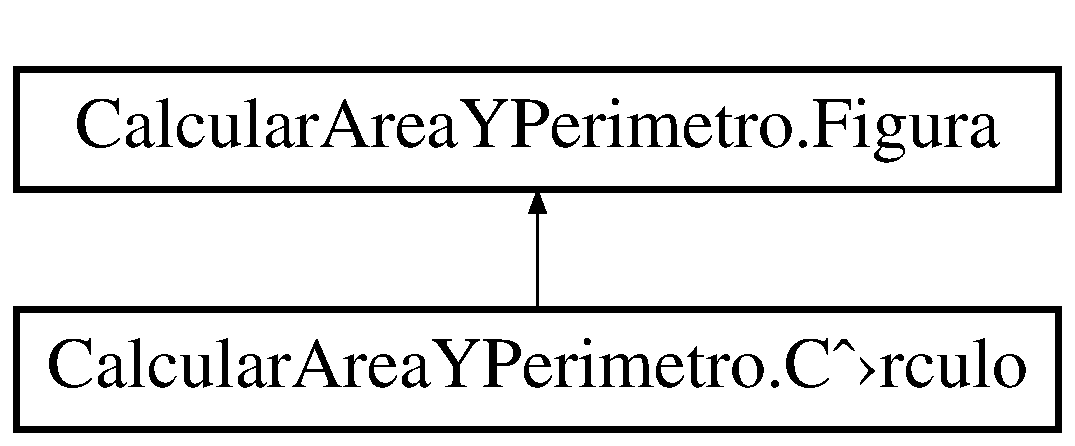
\includegraphics[height=2.000000cm]{class_calcular_area_y_perimetro_1_1_c_xC3_xADrculo}
\end{center}
\end{figure}
\subsection*{Public Member Functions}
\begin{DoxyCompactItemize}
\item 
override float \hyperlink{class_calcular_area_y_perimetro_1_1_c_xC3_xADrculo_ad9f7ee8d44a155b4650194d4c927be08}{Area} ()
\begin{DoxyCompactList}\small\item\em Metodo que calcula el área de un círculo, siendo el radio elevado al cuadrado por el numero P\+I. \end{DoxyCompactList}\item 
override float \hyperlink{class_calcular_area_y_perimetro_1_1_c_xC3_xADrculo_a238460f007f422c1513875f28ba197c7}{Perimeter} ()
\begin{DoxyCompactList}\small\item\em Metodo que calcula el périmetro de un círculo, siendo el producto del radio por P\+I por dos. \end{DoxyCompactList}\end{DoxyCompactItemize}
\subsection*{Properties}
\begin{DoxyCompactItemize}
\item 
float \hyperlink{class_calcular_area_y_perimetro_1_1_c_xC3_xADrculo_a05c05d0c447cd6e28cd3a2d3e52ebd69}{Radio}\hspace{0.3cm}{\ttfamily  \mbox{[}set\mbox{]}}
\begin{DoxyCompactList}\small\item\em Set para el radio del círculo. Si se intenta introducir un valor negativo la variable sera 0. \end{DoxyCompactList}\end{DoxyCompactItemize}


\subsection{Detailed Description}
Clase \hyperlink{class_calcular_area_y_perimetro_1_1_c_xC3_xADrculo}{Círculo} que hereda de la Clase \hyperlink{class_calcular_area_y_perimetro_1_1_figura}{Figura}, permite calcular el area y el perimetro de un círculo. 



\subsection{Member Function Documentation}
\hypertarget{class_calcular_area_y_perimetro_1_1_c_xC3_xADrculo_ad9f7ee8d44a155b4650194d4c927be08}{}\index{Calcular\+Area\+Y\+Perimetro\+::\+Círculo@{Calcular\+Area\+Y\+Perimetro\+::\+Círculo}!Area@{Area}}
\index{Area@{Area}!Calcular\+Area\+Y\+Perimetro\+::\+Círculo@{Calcular\+Area\+Y\+Perimetro\+::\+Círculo}}
\subsubsection[{Area}]{\setlength{\rightskip}{0pt plus 5cm}override float Calcular\+Area\+Y\+Perimetro.\+Círculo.\+Area (
\begin{DoxyParamCaption}
{}
\end{DoxyParamCaption}
)\hspace{0.3cm}{\ttfamily [virtual]}}\label{class_calcular_area_y_perimetro_1_1_c_xC3_xADrculo_ad9f7ee8d44a155b4650194d4c927be08}


Metodo que calcula el área de un círculo, siendo el radio elevado al cuadrado por el numero P\+I. 

\begin{DoxyReturn}{Returns}
Devuele el valor calculado del perímetro en float.
\end{DoxyReturn}


Reimplemented from \hyperlink{class_calcular_area_y_perimetro_1_1_figura_a283e25acf28cd02036270291bdfa99fb}{Calcular\+Area\+Y\+Perimetro.\+Figura}.

\hypertarget{class_calcular_area_y_perimetro_1_1_c_xC3_xADrculo_a238460f007f422c1513875f28ba197c7}{}\index{Calcular\+Area\+Y\+Perimetro\+::\+Círculo@{Calcular\+Area\+Y\+Perimetro\+::\+Círculo}!Perimeter@{Perimeter}}
\index{Perimeter@{Perimeter}!Calcular\+Area\+Y\+Perimetro\+::\+Círculo@{Calcular\+Area\+Y\+Perimetro\+::\+Círculo}}
\subsubsection[{Perimeter}]{\setlength{\rightskip}{0pt plus 5cm}override float Calcular\+Area\+Y\+Perimetro.\+Círculo.\+Perimeter (
\begin{DoxyParamCaption}
{}
\end{DoxyParamCaption}
)\hspace{0.3cm}{\ttfamily [virtual]}}\label{class_calcular_area_y_perimetro_1_1_c_xC3_xADrculo_a238460f007f422c1513875f28ba197c7}


Metodo que calcula el périmetro de un círculo, siendo el producto del radio por P\+I por dos. 

\begin{DoxyReturn}{Returns}
Devuele el valor calculado del área en float.
\end{DoxyReturn}


Reimplemented from \hyperlink{class_calcular_area_y_perimetro_1_1_figura_a501d20cb8d81cdbb12e0dadc48ba2f87}{Calcular\+Area\+Y\+Perimetro.\+Figura}.



\subsection{Property Documentation}
\hypertarget{class_calcular_area_y_perimetro_1_1_c_xC3_xADrculo_a05c05d0c447cd6e28cd3a2d3e52ebd69}{}\index{Calcular\+Area\+Y\+Perimetro\+::\+Círculo@{Calcular\+Area\+Y\+Perimetro\+::\+Círculo}!Radio@{Radio}}
\index{Radio@{Radio}!Calcular\+Area\+Y\+Perimetro\+::\+Círculo@{Calcular\+Area\+Y\+Perimetro\+::\+Círculo}}
\subsubsection[{Radio}]{\setlength{\rightskip}{0pt plus 5cm}float Calcular\+Area\+Y\+Perimetro.\+Círculo.\+Radio\hspace{0.3cm}{\ttfamily [set]}}\label{class_calcular_area_y_perimetro_1_1_c_xC3_xADrculo_a05c05d0c447cd6e28cd3a2d3e52ebd69}


Set para el radio del círculo. Si se intenta introducir un valor negativo la variable sera 0. 



The documentation for this class was generated from the following file\+:\begin{DoxyCompactItemize}
\item 
Calcular\+Perimetro\+Y\+Area/\hyperlink{_c_xC3_xADrculo_8cs}{Círculo.\+cs}\end{DoxyCompactItemize}

\hypertarget{class_calcular_area_y_perimetro_1_1_figura}{}\section{Calcular\+Area\+Y\+Perimetro.\+Figura Class Reference}
\label{class_calcular_area_y_perimetro_1_1_figura}\index{Calcular\+Area\+Y\+Perimetro.\+Figura@{Calcular\+Area\+Y\+Perimetro.\+Figura}}


Clase \hyperlink{class_calcular_area_y_perimetro_1_1_figura}{Figura} de la cual heredarán las demas clases (triángulo, rectángulo y círculo) y que contiene los metodos virtuale que luego sobreescribirán sus hijos para calcular el perímetro y el área.  


Inheritance diagram for Calcular\+Area\+Y\+Perimetro.\+Figura\+:\begin{figure}[H]
\begin{center}
\leavevmode
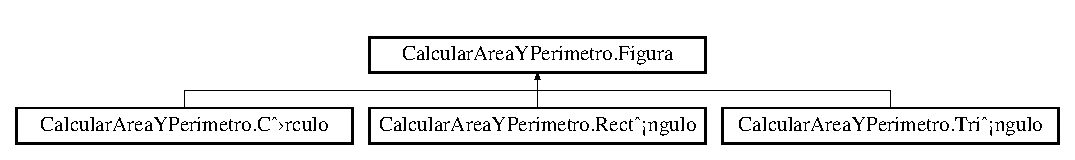
\includegraphics[height=1.696970cm]{class_calcular_area_y_perimetro_1_1_figura}
\end{center}
\end{figure}
\subsection*{Public Member Functions}
\begin{DoxyCompactItemize}
\item 
virtual float \hyperlink{class_calcular_area_y_perimetro_1_1_figura_a501d20cb8d81cdbb12e0dadc48ba2f87}{Perimeter} ()
\begin{DoxyCompactList}\small\item\em Metodo que sera heredado por los hijos para calcular el perímetro de cada uno de ellos. Sera un metodo vacio ya que la clase figura nunca sera usada y solo necesitamos que los hijos hereden el metodo. \end{DoxyCompactList}\item 
virtual float \hyperlink{class_calcular_area_y_perimetro_1_1_figura_a283e25acf28cd02036270291bdfa99fb}{Area} ()
\begin{DoxyCompactList}\small\item\em Metodo que sera heredado por los hijos para calcular el area de cada uno de ellos. Sera un metodo vacio ya que la clase figura nunca sera usada y solo necesitamos que los hijos obtengan el metodo. \end{DoxyCompactList}\end{DoxyCompactItemize}


\subsection{Detailed Description}
Clase \hyperlink{class_calcular_area_y_perimetro_1_1_figura}{Figura} de la cual heredarán las demas clases (triángulo, rectángulo y círculo) y que contiene los metodos virtuale que luego sobreescribirán sus hijos para calcular el perímetro y el área. 



\subsection{Member Function Documentation}
\hypertarget{class_calcular_area_y_perimetro_1_1_figura_a283e25acf28cd02036270291bdfa99fb}{}\index{Calcular\+Area\+Y\+Perimetro\+::\+Figura@{Calcular\+Area\+Y\+Perimetro\+::\+Figura}!Area@{Area}}
\index{Area@{Area}!Calcular\+Area\+Y\+Perimetro\+::\+Figura@{Calcular\+Area\+Y\+Perimetro\+::\+Figura}}
\subsubsection[{Area}]{\setlength{\rightskip}{0pt plus 5cm}virtual float Calcular\+Area\+Y\+Perimetro.\+Figura.\+Area (
\begin{DoxyParamCaption}
{}
\end{DoxyParamCaption}
)\hspace{0.3cm}{\ttfamily [virtual]}}\label{class_calcular_area_y_perimetro_1_1_figura_a283e25acf28cd02036270291bdfa99fb}


Metodo que sera heredado por los hijos para calcular el area de cada uno de ellos. Sera un metodo vacio ya que la clase figura nunca sera usada y solo necesitamos que los hijos obtengan el metodo. 

\begin{DoxyReturn}{Returns}
Devuelve 0.
\end{DoxyReturn}


Reimplemented in \hyperlink{class_calcular_area_y_perimetro_1_1_tri_xC3_xA1ngulo_a269c17af860a19a59a1476b57a182e82}{Calcular\+Area\+Y\+Perimetro.\+Triángulo}, \hyperlink{class_calcular_area_y_perimetro_1_1_rect_xC3_xA1ngulo_a4c223b8f95133eb0522b0986d982cc90}{Calcular\+Area\+Y\+Perimetro.\+Rectángulo}, and \hyperlink{class_calcular_area_y_perimetro_1_1_c_xC3_xADrculo_ad9f7ee8d44a155b4650194d4c927be08}{Calcular\+Area\+Y\+Perimetro.\+Círculo}.

\hypertarget{class_calcular_area_y_perimetro_1_1_figura_a501d20cb8d81cdbb12e0dadc48ba2f87}{}\index{Calcular\+Area\+Y\+Perimetro\+::\+Figura@{Calcular\+Area\+Y\+Perimetro\+::\+Figura}!Perimeter@{Perimeter}}
\index{Perimeter@{Perimeter}!Calcular\+Area\+Y\+Perimetro\+::\+Figura@{Calcular\+Area\+Y\+Perimetro\+::\+Figura}}
\subsubsection[{Perimeter}]{\setlength{\rightskip}{0pt plus 5cm}virtual float Calcular\+Area\+Y\+Perimetro.\+Figura.\+Perimeter (
\begin{DoxyParamCaption}
{}
\end{DoxyParamCaption}
)\hspace{0.3cm}{\ttfamily [virtual]}}\label{class_calcular_area_y_perimetro_1_1_figura_a501d20cb8d81cdbb12e0dadc48ba2f87}


Metodo que sera heredado por los hijos para calcular el perímetro de cada uno de ellos. Sera un metodo vacio ya que la clase figura nunca sera usada y solo necesitamos que los hijos hereden el metodo. 

\begin{DoxyReturn}{Returns}
Devuelve 0.
\end{DoxyReturn}


Reimplemented in \hyperlink{class_calcular_area_y_perimetro_1_1_c_xC3_xADrculo_a238460f007f422c1513875f28ba197c7}{Calcular\+Area\+Y\+Perimetro.\+Círculo}, \hyperlink{class_calcular_area_y_perimetro_1_1_tri_xC3_xA1ngulo_aac49654dd9b222bf2c05daa361b9c454}{Calcular\+Area\+Y\+Perimetro.\+Triángulo}, and \hyperlink{class_calcular_area_y_perimetro_1_1_rect_xC3_xA1ngulo_ab88b945d80ab84beb97d5bf75d757bf2}{Calcular\+Area\+Y\+Perimetro.\+Rectángulo}.



The documentation for this class was generated from the following file\+:\begin{DoxyCompactItemize}
\item 
Calcular\+Perimetro\+Y\+Area/\hyperlink{_figura_8cs}{Figura.\+cs}\end{DoxyCompactItemize}

\hypertarget{class_calcular_perimetro_y_area_1_1_form1}{}\section{Calcular\+Perimetro\+Y\+Area.\+Form1 Class Reference}
\label{class_calcular_perimetro_y_area_1_1_form1}\index{Calcular\+Perimetro\+Y\+Area.\+Form1@{Calcular\+Perimetro\+Y\+Area.\+Form1}}


Clase que servirá como vista nueva para el triángulo, se encargara de recoger los datos del usuario y mandarlos a un objeto de la figura. Es llamada desde el form principal.  


Inheritance diagram for Calcular\+Perimetro\+Y\+Area.\+Form1\+:\begin{figure}[H]
\begin{center}
\leavevmode
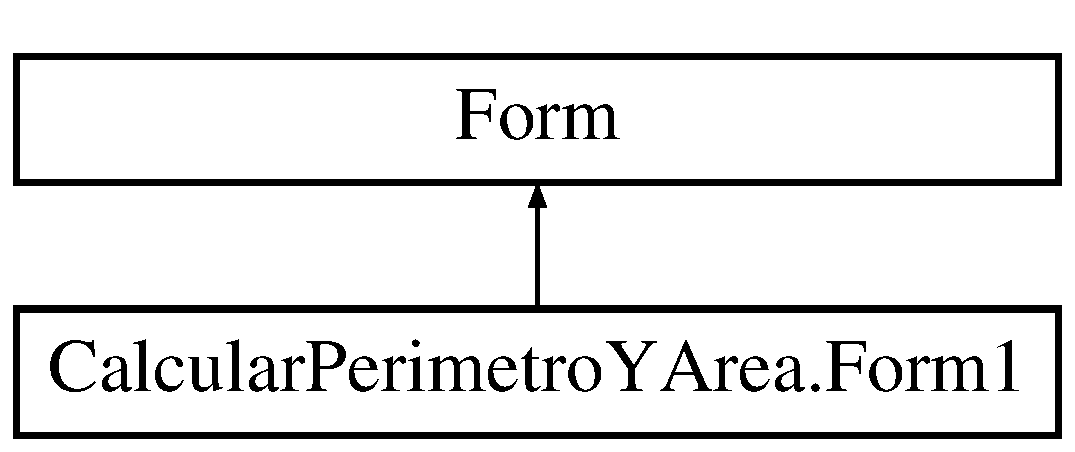
\includegraphics[height=2.000000cm]{class_calcular_perimetro_y_area_1_1_form1}
\end{center}
\end{figure}
\subsection*{Public Member Functions}
\begin{DoxyCompactItemize}
\item 
\hyperlink{class_calcular_perimetro_y_area_1_1_form1_a484d4838e3f6735971072a9257334d91}{Form1} ()
\begin{DoxyCompactList}\small\item\em Metodo que inicializa los componentes. \end{DoxyCompactList}\end{DoxyCompactItemize}
\subsection*{Protected Member Functions}
\begin{DoxyCompactItemize}
\item 
override void \hyperlink{class_calcular_perimetro_y_area_1_1_form1_a4e913ec7eb241ef442a648655cdd93ba}{Dispose} (bool disposing)
\begin{DoxyCompactList}\small\item\em Limpiar los recursos que se estén usando. \end{DoxyCompactList}\end{DoxyCompactItemize}


\subsection{Detailed Description}
Clase que servirá como vista nueva para el triángulo, se encargara de recoger los datos del usuario y mandarlos a un objeto de la figura. Es llamada desde el form principal. 



\subsection{Constructor \& Destructor Documentation}
\hypertarget{class_calcular_perimetro_y_area_1_1_form1_a484d4838e3f6735971072a9257334d91}{}\index{Calcular\+Perimetro\+Y\+Area\+::\+Form1@{Calcular\+Perimetro\+Y\+Area\+::\+Form1}!Form1@{Form1}}
\index{Form1@{Form1}!Calcular\+Perimetro\+Y\+Area\+::\+Form1@{Calcular\+Perimetro\+Y\+Area\+::\+Form1}}
\subsubsection[{Form1}]{\setlength{\rightskip}{0pt plus 5cm}Calcular\+Perimetro\+Y\+Area.\+Form1.\+Form1 (
\begin{DoxyParamCaption}
{}
\end{DoxyParamCaption}
)}\label{class_calcular_perimetro_y_area_1_1_form1_a484d4838e3f6735971072a9257334d91}


Metodo que inicializa los componentes. 



\subsection{Member Function Documentation}
\hypertarget{class_calcular_perimetro_y_area_1_1_form1_a4e913ec7eb241ef442a648655cdd93ba}{}\index{Calcular\+Perimetro\+Y\+Area\+::\+Form1@{Calcular\+Perimetro\+Y\+Area\+::\+Form1}!Dispose@{Dispose}}
\index{Dispose@{Dispose}!Calcular\+Perimetro\+Y\+Area\+::\+Form1@{Calcular\+Perimetro\+Y\+Area\+::\+Form1}}
\subsubsection[{Dispose}]{\setlength{\rightskip}{0pt plus 5cm}override void Calcular\+Perimetro\+Y\+Area.\+Form1.\+Dispose (
\begin{DoxyParamCaption}
\item[{bool}]{disposing}
\end{DoxyParamCaption}
)\hspace{0.3cm}{\ttfamily [protected]}}\label{class_calcular_perimetro_y_area_1_1_form1_a4e913ec7eb241ef442a648655cdd93ba}


Limpiar los recursos que se estén usando. 


\begin{DoxyParams}{Parameters}
{\em disposing} & true si los recursos administrados se deben desechar; false en caso contrario.\\
\hline
\end{DoxyParams}


The documentation for this class was generated from the following files\+:\begin{DoxyCompactItemize}
\item 
Calcular\+Perimetro\+Y\+Area/\hyperlink{_form1_01-_01_copia_8_designer_8cs}{Form1 -\/ Copia.\+Designer.\+cs}\item 
Calcular\+Perimetro\+Y\+Area/\hyperlink{_form1_8cs}{Form1.\+cs}\end{DoxyCompactItemize}

\hypertarget{class_calcular_perimetro_y_area_1_1_form2}{}\section{Calcular\+Perimetro\+Y\+Area.\+Form2 Class Reference}
\label{class_calcular_perimetro_y_area_1_1_form2}\index{Calcular\+Perimetro\+Y\+Area.\+Form2@{Calcular\+Perimetro\+Y\+Area.\+Form2}}


Clase que servirá como vista nueva para el rectángulo, se encargara de recoger los datos del usuario y mandarlos a un objeto de la figura. Es llamada desde el form principal.  


Inheritance diagram for Calcular\+Perimetro\+Y\+Area.\+Form2\+:\begin{figure}[H]
\begin{center}
\leavevmode
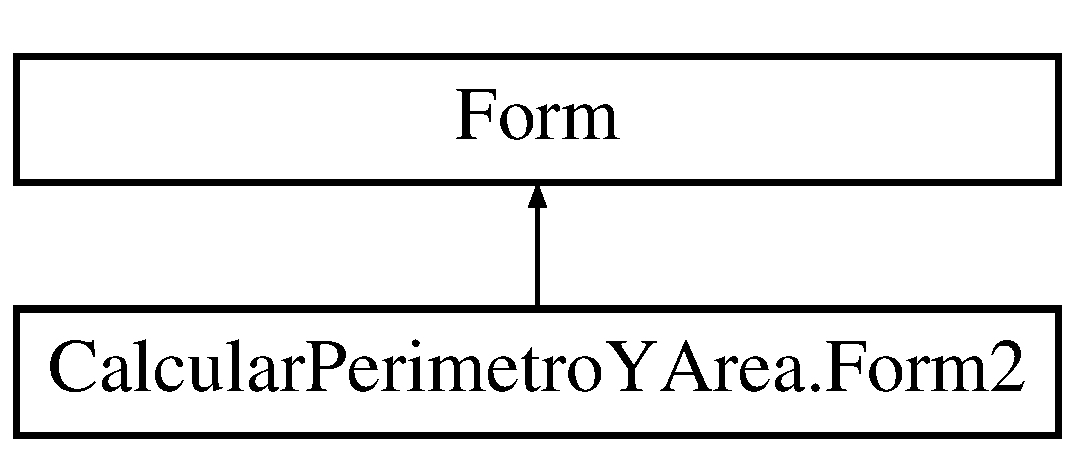
\includegraphics[height=2.000000cm]{class_calcular_perimetro_y_area_1_1_form2}
\end{center}
\end{figure}
\subsection*{Public Member Functions}
\begin{DoxyCompactItemize}
\item 
\hyperlink{class_calcular_perimetro_y_area_1_1_form2_af7f93de70f5e8e88bb24978e7a8839c4}{Form2} ()
\begin{DoxyCompactList}\small\item\em Metodo que inicializa los componentes. \end{DoxyCompactList}\end{DoxyCompactItemize}
\subsection*{Protected Member Functions}
\begin{DoxyCompactItemize}
\item 
override void \hyperlink{class_calcular_perimetro_y_area_1_1_form2_a8607aa1e56e361b157170961294bd971}{Dispose} (bool disposing)
\begin{DoxyCompactList}\small\item\em Clean up any resources being used. \end{DoxyCompactList}\end{DoxyCompactItemize}


\subsection{Detailed Description}
Clase que servirá como vista nueva para el rectángulo, se encargara de recoger los datos del usuario y mandarlos a un objeto de la figura. Es llamada desde el form principal. 



\subsection{Constructor \& Destructor Documentation}
\hypertarget{class_calcular_perimetro_y_area_1_1_form2_af7f93de70f5e8e88bb24978e7a8839c4}{}\index{Calcular\+Perimetro\+Y\+Area\+::\+Form2@{Calcular\+Perimetro\+Y\+Area\+::\+Form2}!Form2@{Form2}}
\index{Form2@{Form2}!Calcular\+Perimetro\+Y\+Area\+::\+Form2@{Calcular\+Perimetro\+Y\+Area\+::\+Form2}}
\subsubsection[{Form2}]{\setlength{\rightskip}{0pt plus 5cm}Calcular\+Perimetro\+Y\+Area.\+Form2.\+Form2 (
\begin{DoxyParamCaption}
{}
\end{DoxyParamCaption}
)}\label{class_calcular_perimetro_y_area_1_1_form2_af7f93de70f5e8e88bb24978e7a8839c4}


Metodo que inicializa los componentes. 



\subsection{Member Function Documentation}
\hypertarget{class_calcular_perimetro_y_area_1_1_form2_a8607aa1e56e361b157170961294bd971}{}\index{Calcular\+Perimetro\+Y\+Area\+::\+Form2@{Calcular\+Perimetro\+Y\+Area\+::\+Form2}!Dispose@{Dispose}}
\index{Dispose@{Dispose}!Calcular\+Perimetro\+Y\+Area\+::\+Form2@{Calcular\+Perimetro\+Y\+Area\+::\+Form2}}
\subsubsection[{Dispose}]{\setlength{\rightskip}{0pt plus 5cm}override void Calcular\+Perimetro\+Y\+Area.\+Form2.\+Dispose (
\begin{DoxyParamCaption}
\item[{bool}]{disposing}
\end{DoxyParamCaption}
)\hspace{0.3cm}{\ttfamily [protected]}}\label{class_calcular_perimetro_y_area_1_1_form2_a8607aa1e56e361b157170961294bd971}


Clean up any resources being used. 


\begin{DoxyParams}{Parameters}
{\em disposing} & true if managed resources should be disposed; otherwise, false.\\
\hline
\end{DoxyParams}


The documentation for this class was generated from the following files\+:\begin{DoxyCompactItemize}
\item 
Calcular\+Perimetro\+Y\+Area/\hyperlink{_form2_8cs}{Form2.\+cs}\item 
Calcular\+Perimetro\+Y\+Area/\hyperlink{_form2_8_designer_8cs}{Form2.\+Designer.\+cs}\end{DoxyCompactItemize}

\hypertarget{class_calcular_perimetro_y_area_1_1_form3}{}\section{Calcular\+Perimetro\+Y\+Area.\+Form3 Class Reference}
\label{class_calcular_perimetro_y_area_1_1_form3}\index{Calcular\+Perimetro\+Y\+Area.\+Form3@{Calcular\+Perimetro\+Y\+Area.\+Form3}}


Clase que servirá como vista nueva para el círculo, se encargara de recoger los datos del usuario y mandarlos a un objeto de la figura. Es llamada desde el form principal.  


Inheritance diagram for Calcular\+Perimetro\+Y\+Area.\+Form3\+:\begin{figure}[H]
\begin{center}
\leavevmode
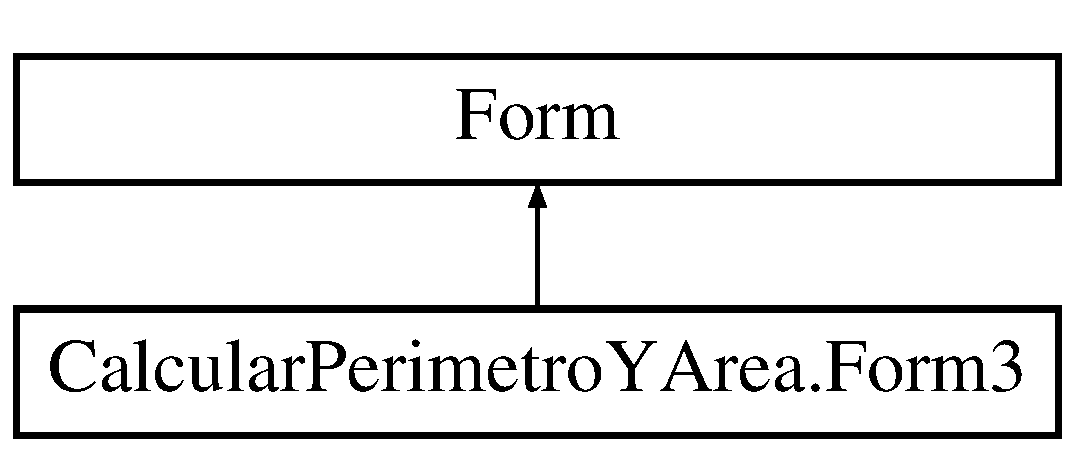
\includegraphics[height=2.000000cm]{class_calcular_perimetro_y_area_1_1_form3}
\end{center}
\end{figure}
\subsection*{Public Member Functions}
\begin{DoxyCompactItemize}
\item 
\hyperlink{class_calcular_perimetro_y_area_1_1_form3_a6ade964c5c2ed1690f66740e44a5b94c}{Form3} ()
\begin{DoxyCompactList}\small\item\em Metodo que inicializa los componentes. \end{DoxyCompactList}\end{DoxyCompactItemize}
\subsection*{Protected Member Functions}
\begin{DoxyCompactItemize}
\item 
override void \hyperlink{class_calcular_perimetro_y_area_1_1_form3_a5a1bbefcee0d410ef7fbceb0d976fa33}{Dispose} (bool disposing)
\begin{DoxyCompactList}\small\item\em Clean up any resources being used. \end{DoxyCompactList}\end{DoxyCompactItemize}


\subsection{Detailed Description}
Clase que servirá como vista nueva para el círculo, se encargara de recoger los datos del usuario y mandarlos a un objeto de la figura. Es llamada desde el form principal. 



\subsection{Constructor \& Destructor Documentation}
\hypertarget{class_calcular_perimetro_y_area_1_1_form3_a6ade964c5c2ed1690f66740e44a5b94c}{}\index{Calcular\+Perimetro\+Y\+Area\+::\+Form3@{Calcular\+Perimetro\+Y\+Area\+::\+Form3}!Form3@{Form3}}
\index{Form3@{Form3}!Calcular\+Perimetro\+Y\+Area\+::\+Form3@{Calcular\+Perimetro\+Y\+Area\+::\+Form3}}
\subsubsection[{Form3}]{\setlength{\rightskip}{0pt plus 5cm}Calcular\+Perimetro\+Y\+Area.\+Form3.\+Form3 (
\begin{DoxyParamCaption}
{}
\end{DoxyParamCaption}
)}\label{class_calcular_perimetro_y_area_1_1_form3_a6ade964c5c2ed1690f66740e44a5b94c}


Metodo que inicializa los componentes. 



\subsection{Member Function Documentation}
\hypertarget{class_calcular_perimetro_y_area_1_1_form3_a5a1bbefcee0d410ef7fbceb0d976fa33}{}\index{Calcular\+Perimetro\+Y\+Area\+::\+Form3@{Calcular\+Perimetro\+Y\+Area\+::\+Form3}!Dispose@{Dispose}}
\index{Dispose@{Dispose}!Calcular\+Perimetro\+Y\+Area\+::\+Form3@{Calcular\+Perimetro\+Y\+Area\+::\+Form3}}
\subsubsection[{Dispose}]{\setlength{\rightskip}{0pt plus 5cm}override void Calcular\+Perimetro\+Y\+Area.\+Form3.\+Dispose (
\begin{DoxyParamCaption}
\item[{bool}]{disposing}
\end{DoxyParamCaption}
)\hspace{0.3cm}{\ttfamily [protected]}}\label{class_calcular_perimetro_y_area_1_1_form3_a5a1bbefcee0d410ef7fbceb0d976fa33}


Clean up any resources being used. 


\begin{DoxyParams}{Parameters}
{\em disposing} & true if managed resources should be disposed; otherwise, false.\\
\hline
\end{DoxyParams}


The documentation for this class was generated from the following files\+:\begin{DoxyCompactItemize}
\item 
Calcular\+Perimetro\+Y\+Area/\hyperlink{_form3_8cs}{Form3.\+cs}\item 
Calcular\+Perimetro\+Y\+Area/\hyperlink{_form3_8_designer_8cs}{Form3.\+Designer.\+cs}\end{DoxyCompactItemize}

\hypertarget{class_calcular_perimetro_y_area_1_1form_principal}{}\section{Calcular\+Perimetro\+Y\+Area.\+form\+Principal Class Reference}
\label{class_calcular_perimetro_y_area_1_1form_principal}\index{Calcular\+Perimetro\+Y\+Area.\+form\+Principal@{Calcular\+Perimetro\+Y\+Area.\+form\+Principal}}


Clase que será la vista principal del programa, en el elegiremos para que figura queremos calcular el área y el périmetro.  


Inheritance diagram for Calcular\+Perimetro\+Y\+Area.\+form\+Principal\+:\begin{figure}[H]
\begin{center}
\leavevmode
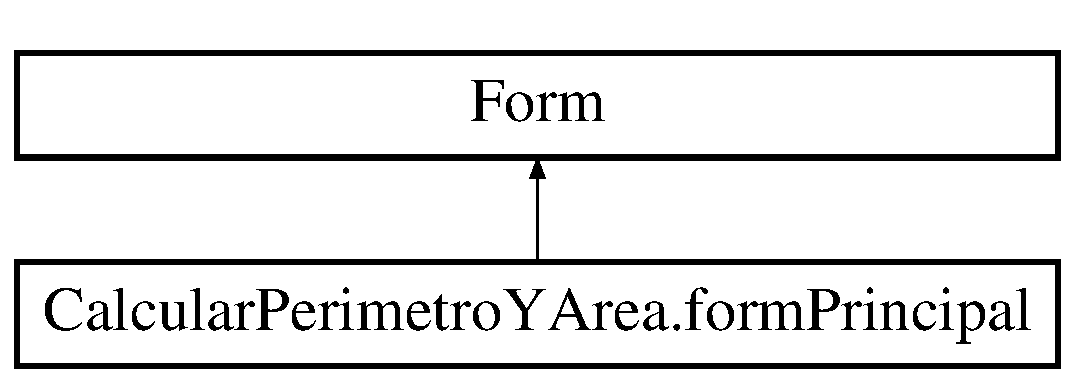
\includegraphics[height=2.000000cm]{class_calcular_perimetro_y_area_1_1form_principal}
\end{center}
\end{figure}
\subsection*{Public Member Functions}
\begin{DoxyCompactItemize}
\item 
\hyperlink{class_calcular_perimetro_y_area_1_1form_principal_a6a27d2db038189fc9856ce958495ffd0}{form\+Principal} ()
\begin{DoxyCompactList}\small\item\em Metodo que inicializa los componentes. \end{DoxyCompactList}\end{DoxyCompactItemize}
\subsection*{Protected Member Functions}
\begin{DoxyCompactItemize}
\item 
override void \hyperlink{class_calcular_perimetro_y_area_1_1form_principal_aa215d44c5c947aedfec46f810d0120dc}{Dispose} (bool disposing)
\begin{DoxyCompactList}\small\item\em Clean up any resources being used. \end{DoxyCompactList}\end{DoxyCompactItemize}


\subsection{Detailed Description}
Clase que será la vista principal del programa, en el elegiremos para que figura queremos calcular el área y el périmetro. 



\subsection{Constructor \& Destructor Documentation}
\hypertarget{class_calcular_perimetro_y_area_1_1form_principal_a6a27d2db038189fc9856ce958495ffd0}{}\index{Calcular\+Perimetro\+Y\+Area\+::form\+Principal@{Calcular\+Perimetro\+Y\+Area\+::form\+Principal}!form\+Principal@{form\+Principal}}
\index{form\+Principal@{form\+Principal}!Calcular\+Perimetro\+Y\+Area\+::form\+Principal@{Calcular\+Perimetro\+Y\+Area\+::form\+Principal}}
\subsubsection[{form\+Principal}]{\setlength{\rightskip}{0pt plus 5cm}Calcular\+Perimetro\+Y\+Area.\+form\+Principal.\+form\+Principal (
\begin{DoxyParamCaption}
{}
\end{DoxyParamCaption}
)}\label{class_calcular_perimetro_y_area_1_1form_principal_a6a27d2db038189fc9856ce958495ffd0}


Metodo que inicializa los componentes. 



\subsection{Member Function Documentation}
\hypertarget{class_calcular_perimetro_y_area_1_1form_principal_aa215d44c5c947aedfec46f810d0120dc}{}\index{Calcular\+Perimetro\+Y\+Area\+::form\+Principal@{Calcular\+Perimetro\+Y\+Area\+::form\+Principal}!Dispose@{Dispose}}
\index{Dispose@{Dispose}!Calcular\+Perimetro\+Y\+Area\+::form\+Principal@{Calcular\+Perimetro\+Y\+Area\+::form\+Principal}}
\subsubsection[{Dispose}]{\setlength{\rightskip}{0pt plus 5cm}override void Calcular\+Perimetro\+Y\+Area.\+form\+Principal.\+Dispose (
\begin{DoxyParamCaption}
\item[{bool}]{disposing}
\end{DoxyParamCaption}
)\hspace{0.3cm}{\ttfamily [protected]}}\label{class_calcular_perimetro_y_area_1_1form_principal_aa215d44c5c947aedfec46f810d0120dc}


Clean up any resources being used. 


\begin{DoxyParams}{Parameters}
{\em disposing} & true if managed resources should be disposed; otherwise, false.\\
\hline
\end{DoxyParams}


The documentation for this class was generated from the following files\+:\begin{DoxyCompactItemize}
\item 
Calcular\+Perimetro\+Y\+Area/\hyperlink{_form_principal_8cs}{Form\+Principal.\+cs}\item 
Calcular\+Perimetro\+Y\+Area/\hyperlink{_form_principal_8_designer_8cs}{Form\+Principal.\+Designer.\+cs}\end{DoxyCompactItemize}

\hypertarget{class_calcular_area_y_perimetro_1_1_rect_xC3_xA1ngulo}{}\section{Calcular\+Area\+Y\+Perimetro.\+Rectángulo Class Reference}
\label{class_calcular_area_y_perimetro_1_1_rect_xC3_xA1ngulo}\index{Calcular\+Area\+Y\+Perimetro.\+Rectángulo@{Calcular\+Area\+Y\+Perimetro.\+Rectángulo}}


Clase \hyperlink{class_calcular_area_y_perimetro_1_1_rect_xC3_xA1ngulo}{Rectángulo} que hereda de la Clase \hyperlink{class_calcular_area_y_perimetro_1_1_figura}{Figura}, permite calcular el area y el perimetro de un rectangulo.  


Inheritance diagram for Calcular\+Area\+Y\+Perimetro.\+Rectángulo\+:\begin{figure}[H]
\begin{center}
\leavevmode
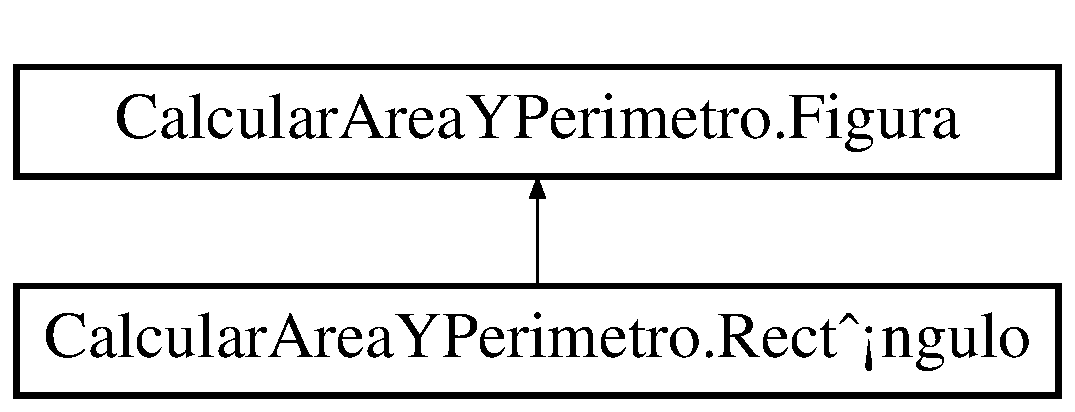
\includegraphics[height=2.000000cm]{class_calcular_area_y_perimetro_1_1_rect_xC3_xA1ngulo}
\end{center}
\end{figure}
\subsection*{Public Member Functions}
\begin{DoxyCompactItemize}
\item 
override float \hyperlink{class_calcular_area_y_perimetro_1_1_rect_xC3_xA1ngulo_ab88b945d80ab84beb97d5bf75d757bf2}{Perimeter} ()
\begin{DoxyCompactList}\small\item\em Metodo de tipo Float que permite calcular el área de un rectángulo, siendo la suma de la base y la altura por dos. \end{DoxyCompactList}\item 
override float \hyperlink{class_calcular_area_y_perimetro_1_1_rect_xC3_xA1ngulo_a4c223b8f95133eb0522b0986d982cc90}{Area} ()
\begin{DoxyCompactList}\small\item\em Metodo de tipo Float que permite calcular el área de un rectángulo, siendo el producto de la altura y la base. \end{DoxyCompactList}\end{DoxyCompactItemize}
\subsection*{Properties}
\begin{DoxyCompactItemize}
\item 
float \hyperlink{class_calcular_area_y_perimetro_1_1_rect_xC3_xA1ngulo_a19af4a57456caf9042cca100d3a9bc52}{Weight}\hspace{0.3cm}{\ttfamily  \mbox{[}set\mbox{]}}
\begin{DoxyCompactList}\small\item\em Set para la base del rectángulo. Si se intenta introducir un valor negativo la variable sera 0. \end{DoxyCompactList}\item 
float \hyperlink{class_calcular_area_y_perimetro_1_1_rect_xC3_xA1ngulo_a5b2b03b9dc4ffe23a68e697ecc8fbc91}{Height}\hspace{0.3cm}{\ttfamily  \mbox{[}set\mbox{]}}
\begin{DoxyCompactList}\small\item\em Set para la altura del rectángulo. Si se intenta introducir un valor negativo la variable sera 0. \end{DoxyCompactList}\end{DoxyCompactItemize}


\subsection{Detailed Description}
Clase \hyperlink{class_calcular_area_y_perimetro_1_1_rect_xC3_xA1ngulo}{Rectángulo} que hereda de la Clase \hyperlink{class_calcular_area_y_perimetro_1_1_figura}{Figura}, permite calcular el area y el perimetro de un rectangulo. 



\subsection{Member Function Documentation}
\hypertarget{class_calcular_area_y_perimetro_1_1_rect_xC3_xA1ngulo_a4c223b8f95133eb0522b0986d982cc90}{}\index{Calcular\+Area\+Y\+Perimetro\+::\+Rectángulo@{Calcular\+Area\+Y\+Perimetro\+::\+Rectángulo}!Area@{Area}}
\index{Area@{Area}!Calcular\+Area\+Y\+Perimetro\+::\+Rectángulo@{Calcular\+Area\+Y\+Perimetro\+::\+Rectángulo}}
\subsubsection[{Area}]{\setlength{\rightskip}{0pt plus 5cm}override float Calcular\+Area\+Y\+Perimetro.\+Rectángulo.\+Area (
\begin{DoxyParamCaption}
{}
\end{DoxyParamCaption}
)\hspace{0.3cm}{\ttfamily [virtual]}}\label{class_calcular_area_y_perimetro_1_1_rect_xC3_xA1ngulo_a4c223b8f95133eb0522b0986d982cc90}


Metodo de tipo Float que permite calcular el área de un rectángulo, siendo el producto de la altura y la base. 

\begin{DoxyReturn}{Returns}

\end{DoxyReturn}


Reimplemented from \hyperlink{class_calcular_area_y_perimetro_1_1_figura_a283e25acf28cd02036270291bdfa99fb}{Calcular\+Area\+Y\+Perimetro.\+Figura}.

\hypertarget{class_calcular_area_y_perimetro_1_1_rect_xC3_xA1ngulo_ab88b945d80ab84beb97d5bf75d757bf2}{}\index{Calcular\+Area\+Y\+Perimetro\+::\+Rectángulo@{Calcular\+Area\+Y\+Perimetro\+::\+Rectángulo}!Perimeter@{Perimeter}}
\index{Perimeter@{Perimeter}!Calcular\+Area\+Y\+Perimetro\+::\+Rectángulo@{Calcular\+Area\+Y\+Perimetro\+::\+Rectángulo}}
\subsubsection[{Perimeter}]{\setlength{\rightskip}{0pt plus 5cm}override float Calcular\+Area\+Y\+Perimetro.\+Rectángulo.\+Perimeter (
\begin{DoxyParamCaption}
{}
\end{DoxyParamCaption}
)\hspace{0.3cm}{\ttfamily [virtual]}}\label{class_calcular_area_y_perimetro_1_1_rect_xC3_xA1ngulo_ab88b945d80ab84beb97d5bf75d757bf2}


Metodo de tipo Float que permite calcular el área de un rectángulo, siendo la suma de la base y la altura por dos. 

\begin{DoxyReturn}{Returns}

\end{DoxyReturn}


Reimplemented from \hyperlink{class_calcular_area_y_perimetro_1_1_figura_a501d20cb8d81cdbb12e0dadc48ba2f87}{Calcular\+Area\+Y\+Perimetro.\+Figura}.



\subsection{Property Documentation}
\hypertarget{class_calcular_area_y_perimetro_1_1_rect_xC3_xA1ngulo_a5b2b03b9dc4ffe23a68e697ecc8fbc91}{}\index{Calcular\+Area\+Y\+Perimetro\+::\+Rectángulo@{Calcular\+Area\+Y\+Perimetro\+::\+Rectángulo}!Height@{Height}}
\index{Height@{Height}!Calcular\+Area\+Y\+Perimetro\+::\+Rectángulo@{Calcular\+Area\+Y\+Perimetro\+::\+Rectángulo}}
\subsubsection[{Height}]{\setlength{\rightskip}{0pt plus 5cm}float Calcular\+Area\+Y\+Perimetro.\+Rectángulo.\+Height\hspace{0.3cm}{\ttfamily [set]}}\label{class_calcular_area_y_perimetro_1_1_rect_xC3_xA1ngulo_a5b2b03b9dc4ffe23a68e697ecc8fbc91}


Set para la altura del rectángulo. Si se intenta introducir un valor negativo la variable sera 0. 

\hypertarget{class_calcular_area_y_perimetro_1_1_rect_xC3_xA1ngulo_a19af4a57456caf9042cca100d3a9bc52}{}\index{Calcular\+Area\+Y\+Perimetro\+::\+Rectángulo@{Calcular\+Area\+Y\+Perimetro\+::\+Rectángulo}!Weight@{Weight}}
\index{Weight@{Weight}!Calcular\+Area\+Y\+Perimetro\+::\+Rectángulo@{Calcular\+Area\+Y\+Perimetro\+::\+Rectángulo}}
\subsubsection[{Weight}]{\setlength{\rightskip}{0pt plus 5cm}float Calcular\+Area\+Y\+Perimetro.\+Rectángulo.\+Weight\hspace{0.3cm}{\ttfamily [set]}}\label{class_calcular_area_y_perimetro_1_1_rect_xC3_xA1ngulo_a19af4a57456caf9042cca100d3a9bc52}


Set para la base del rectángulo. Si se intenta introducir un valor negativo la variable sera 0. 



The documentation for this class was generated from the following file\+:\begin{DoxyCompactItemize}
\item 
Calcular\+Perimetro\+Y\+Area/\hyperlink{_rect_xC3_xA1ngulo_8cs}{Rectángulo.\+cs}\end{DoxyCompactItemize}

\hypertarget{class_calcular_area_y_perimetro_1_1_tri_xC3_xA1ngulo}{}\section{Calcular\+Area\+Y\+Perimetro.\+Triángulo Class Reference}
\label{class_calcular_area_y_perimetro_1_1_tri_xC3_xA1ngulo}\index{Calcular\+Area\+Y\+Perimetro.\+Triángulo@{Calcular\+Area\+Y\+Perimetro.\+Triángulo}}


Clase que hace referencia a un triángulo que hereda de la clase \hyperlink{class_calcular_area_y_perimetro_1_1_figura}{Figura} y nos permitira calcular su área y perímetro.  


Inheritance diagram for Calcular\+Area\+Y\+Perimetro.\+Triángulo\+:\begin{figure}[H]
\begin{center}
\leavevmode
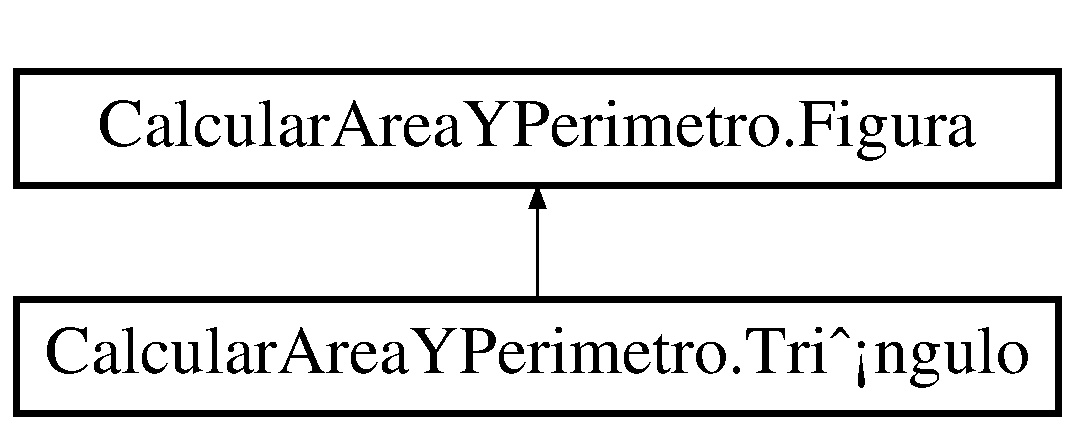
\includegraphics[height=2.000000cm]{class_calcular_area_y_perimetro_1_1_tri_xC3_xA1ngulo}
\end{center}
\end{figure}
\subsection*{Public Member Functions}
\begin{DoxyCompactItemize}
\item 
override float \hyperlink{class_calcular_area_y_perimetro_1_1_tri_xC3_xA1ngulo_aac49654dd9b222bf2c05daa361b9c454}{Perimeter} ()
\begin{DoxyCompactList}\small\item\em Metodo de tipo Float que permite calcular el perímetro de un triángulo, siendo la suma de todos sus lados. \end{DoxyCompactList}\item 
override float \hyperlink{class_calcular_area_y_perimetro_1_1_tri_xC3_xA1ngulo_a269c17af860a19a59a1476b57a182e82}{Area} ()
\begin{DoxyCompactList}\small\item\em Metodo de tipo Float que permite calcular el área de un triángulo, siendo la base por la altura entre dos. \end{DoxyCompactList}\end{DoxyCompactItemize}
\subsection*{Properties}
\begin{DoxyCompactItemize}
\item 
float \hyperlink{class_calcular_area_y_perimetro_1_1_tri_xC3_xA1ngulo_a920ba2504420213af32951b4fb7d6c9b}{Base\+Tri}\hspace{0.3cm}{\ttfamily  \mbox{[}set\mbox{]}}
\begin{DoxyCompactList}\small\item\em Set para la base del triángulo. Si se intenta introducir un valor negativo la variable sera 0. \end{DoxyCompactList}\item 
float \hyperlink{class_calcular_area_y_perimetro_1_1_tri_xC3_xA1ngulo_a03db58b7dc2703d2844fc6391088b891}{Height}\hspace{0.3cm}{\ttfamily  \mbox{[}set\mbox{]}}
\begin{DoxyCompactList}\small\item\em Set para la altura del triángulo. Si se intenta introducir un valor negativo la variable sera 0. \end{DoxyCompactList}\item 
float \hyperlink{class_calcular_area_y_perimetro_1_1_tri_xC3_xA1ngulo_af3c271639fdbaad3825bba7f0490e13b}{A}\hspace{0.3cm}{\ttfamily  \mbox{[}set\mbox{]}}
\begin{DoxyCompactList}\small\item\em Set para el lado A del triángulo. Si se intenta introducir un valor negativo la variable sera 0. \end{DoxyCompactList}\item 
float \hyperlink{class_calcular_area_y_perimetro_1_1_tri_xC3_xA1ngulo_a4112d330d1d2b05fc6a2c21d68dfd9d2}{B}\hspace{0.3cm}{\ttfamily  \mbox{[}set\mbox{]}}
\begin{DoxyCompactList}\small\item\em Set para el lado B del triángulo. Si se intenta introducir un valor negativo la variable sera 0. \end{DoxyCompactList}\item 
float \hyperlink{class_calcular_area_y_perimetro_1_1_tri_xC3_xA1ngulo_a8d249cc94138997fbc0a51a1b54ffd3b}{C}\hspace{0.3cm}{\ttfamily  \mbox{[}set\mbox{]}}
\begin{DoxyCompactList}\small\item\em Set para el lado C del triángulo. Si se intenta introducir un valor negativo la variable sera 0. \end{DoxyCompactList}\end{DoxyCompactItemize}


\subsection{Detailed Description}
Clase que hace referencia a un triángulo que hereda de la clase \hyperlink{class_calcular_area_y_perimetro_1_1_figura}{Figura} y nos permitira calcular su área y perímetro. 



\subsection{Member Function Documentation}
\hypertarget{class_calcular_area_y_perimetro_1_1_tri_xC3_xA1ngulo_a269c17af860a19a59a1476b57a182e82}{}\index{Calcular\+Area\+Y\+Perimetro\+::\+Triángulo@{Calcular\+Area\+Y\+Perimetro\+::\+Triángulo}!Area@{Area}}
\index{Area@{Area}!Calcular\+Area\+Y\+Perimetro\+::\+Triángulo@{Calcular\+Area\+Y\+Perimetro\+::\+Triángulo}}
\subsubsection[{Area}]{\setlength{\rightskip}{0pt plus 5cm}override float Calcular\+Area\+Y\+Perimetro.\+Triángulo.\+Area (
\begin{DoxyParamCaption}
{}
\end{DoxyParamCaption}
)\hspace{0.3cm}{\ttfamily [virtual]}}\label{class_calcular_area_y_perimetro_1_1_tri_xC3_xA1ngulo_a269c17af860a19a59a1476b57a182e82}


Metodo de tipo Float que permite calcular el área de un triángulo, siendo la base por la altura entre dos. 

\begin{DoxyReturn}{Returns}

\end{DoxyReturn}


Reimplemented from \hyperlink{class_calcular_area_y_perimetro_1_1_figura_a283e25acf28cd02036270291bdfa99fb}{Calcular\+Area\+Y\+Perimetro.\+Figura}.

\hypertarget{class_calcular_area_y_perimetro_1_1_tri_xC3_xA1ngulo_aac49654dd9b222bf2c05daa361b9c454}{}\index{Calcular\+Area\+Y\+Perimetro\+::\+Triángulo@{Calcular\+Area\+Y\+Perimetro\+::\+Triángulo}!Perimeter@{Perimeter}}
\index{Perimeter@{Perimeter}!Calcular\+Area\+Y\+Perimetro\+::\+Triángulo@{Calcular\+Area\+Y\+Perimetro\+::\+Triángulo}}
\subsubsection[{Perimeter}]{\setlength{\rightskip}{0pt plus 5cm}override float Calcular\+Area\+Y\+Perimetro.\+Triángulo.\+Perimeter (
\begin{DoxyParamCaption}
{}
\end{DoxyParamCaption}
)\hspace{0.3cm}{\ttfamily [virtual]}}\label{class_calcular_area_y_perimetro_1_1_tri_xC3_xA1ngulo_aac49654dd9b222bf2c05daa361b9c454}


Metodo de tipo Float que permite calcular el perímetro de un triángulo, siendo la suma de todos sus lados. 

\begin{DoxyReturn}{Returns}
Devuelve el valor del perímetro.
\end{DoxyReturn}


Reimplemented from \hyperlink{class_calcular_area_y_perimetro_1_1_figura_a501d20cb8d81cdbb12e0dadc48ba2f87}{Calcular\+Area\+Y\+Perimetro.\+Figura}.



\subsection{Property Documentation}
\hypertarget{class_calcular_area_y_perimetro_1_1_tri_xC3_xA1ngulo_af3c271639fdbaad3825bba7f0490e13b}{}\index{Calcular\+Area\+Y\+Perimetro\+::\+Triángulo@{Calcular\+Area\+Y\+Perimetro\+::\+Triángulo}!A@{A}}
\index{A@{A}!Calcular\+Area\+Y\+Perimetro\+::\+Triángulo@{Calcular\+Area\+Y\+Perimetro\+::\+Triángulo}}
\subsubsection[{A}]{\setlength{\rightskip}{0pt plus 5cm}float Calcular\+Area\+Y\+Perimetro.\+Triángulo.\+A\hspace{0.3cm}{\ttfamily [set]}}\label{class_calcular_area_y_perimetro_1_1_tri_xC3_xA1ngulo_af3c271639fdbaad3825bba7f0490e13b}


Set para el lado A del triángulo. Si se intenta introducir un valor negativo la variable sera 0. 

\hypertarget{class_calcular_area_y_perimetro_1_1_tri_xC3_xA1ngulo_a4112d330d1d2b05fc6a2c21d68dfd9d2}{}\index{Calcular\+Area\+Y\+Perimetro\+::\+Triángulo@{Calcular\+Area\+Y\+Perimetro\+::\+Triángulo}!B@{B}}
\index{B@{B}!Calcular\+Area\+Y\+Perimetro\+::\+Triángulo@{Calcular\+Area\+Y\+Perimetro\+::\+Triángulo}}
\subsubsection[{B}]{\setlength{\rightskip}{0pt plus 5cm}float Calcular\+Area\+Y\+Perimetro.\+Triángulo.\+B\hspace{0.3cm}{\ttfamily [set]}}\label{class_calcular_area_y_perimetro_1_1_tri_xC3_xA1ngulo_a4112d330d1d2b05fc6a2c21d68dfd9d2}


Set para el lado B del triángulo. Si se intenta introducir un valor negativo la variable sera 0. 

\hypertarget{class_calcular_area_y_perimetro_1_1_tri_xC3_xA1ngulo_a920ba2504420213af32951b4fb7d6c9b}{}\index{Calcular\+Area\+Y\+Perimetro\+::\+Triángulo@{Calcular\+Area\+Y\+Perimetro\+::\+Triángulo}!Base\+Tri@{Base\+Tri}}
\index{Base\+Tri@{Base\+Tri}!Calcular\+Area\+Y\+Perimetro\+::\+Triángulo@{Calcular\+Area\+Y\+Perimetro\+::\+Triángulo}}
\subsubsection[{Base\+Tri}]{\setlength{\rightskip}{0pt plus 5cm}float Calcular\+Area\+Y\+Perimetro.\+Triángulo.\+Base\+Tri\hspace{0.3cm}{\ttfamily [set]}}\label{class_calcular_area_y_perimetro_1_1_tri_xC3_xA1ngulo_a920ba2504420213af32951b4fb7d6c9b}


Set para la base del triángulo. Si se intenta introducir un valor negativo la variable sera 0. 

\hypertarget{class_calcular_area_y_perimetro_1_1_tri_xC3_xA1ngulo_a8d249cc94138997fbc0a51a1b54ffd3b}{}\index{Calcular\+Area\+Y\+Perimetro\+::\+Triángulo@{Calcular\+Area\+Y\+Perimetro\+::\+Triángulo}!C@{C}}
\index{C@{C}!Calcular\+Area\+Y\+Perimetro\+::\+Triángulo@{Calcular\+Area\+Y\+Perimetro\+::\+Triángulo}}
\subsubsection[{C}]{\setlength{\rightskip}{0pt plus 5cm}float Calcular\+Area\+Y\+Perimetro.\+Triángulo.\+C\hspace{0.3cm}{\ttfamily [set]}}\label{class_calcular_area_y_perimetro_1_1_tri_xC3_xA1ngulo_a8d249cc94138997fbc0a51a1b54ffd3b}


Set para el lado C del triángulo. Si se intenta introducir un valor negativo la variable sera 0. 

\hypertarget{class_calcular_area_y_perimetro_1_1_tri_xC3_xA1ngulo_a03db58b7dc2703d2844fc6391088b891}{}\index{Calcular\+Area\+Y\+Perimetro\+::\+Triángulo@{Calcular\+Area\+Y\+Perimetro\+::\+Triángulo}!Height@{Height}}
\index{Height@{Height}!Calcular\+Area\+Y\+Perimetro\+::\+Triángulo@{Calcular\+Area\+Y\+Perimetro\+::\+Triángulo}}
\subsubsection[{Height}]{\setlength{\rightskip}{0pt plus 5cm}float Calcular\+Area\+Y\+Perimetro.\+Triángulo.\+Height\hspace{0.3cm}{\ttfamily [set]}}\label{class_calcular_area_y_perimetro_1_1_tri_xC3_xA1ngulo_a03db58b7dc2703d2844fc6391088b891}


Set para la altura del triángulo. Si se intenta introducir un valor negativo la variable sera 0. 



The documentation for this class was generated from the following file\+:\begin{DoxyCompactItemize}
\item 
Calcular\+Perimetro\+Y\+Area/\hyperlink{_tri_xC3_xA1ngulo_8cs}{Triángulo.\+cs}\end{DoxyCompactItemize}

\chapter{File Documentation}
\hypertarget{_c_xC3_xADrculo_8cs}{}\section{Calcular\+Perimetro\+Y\+Area/\+Círculo.cs File Reference}
\label{_c_xC3_xADrculo_8cs}\index{Calcular\+Perimetro\+Y\+Area/\+Círculo.\+cs@{Calcular\+Perimetro\+Y\+Area/\+Círculo.\+cs}}
\subsection*{Classes}
\begin{DoxyCompactItemize}
\item 
class \hyperlink{class_calcular_area_y_perimetro_1_1_c_xC3_xADrculo}{Calcular\+Area\+Y\+Perimetro.\+Círculo}
\begin{DoxyCompactList}\small\item\em Clase \hyperlink{class_calcular_area_y_perimetro_1_1_c_xC3_xADrculo}{Círculo} que hereda de la Clase \hyperlink{class_calcular_area_y_perimetro_1_1_figura}{Figura}, permite calcular el area y el perimetro de un círculo. \end{DoxyCompactList}\end{DoxyCompactItemize}
\subsection*{Namespaces}
\begin{DoxyCompactItemize}
\item 
package \hyperlink{namespace_calcular_area_y_perimetro}{Calcular\+Area\+Y\+Perimetro}
\end{DoxyCompactItemize}

\hypertarget{_figura_8cs}{}\section{Calcular\+Perimetro\+Y\+Area/\+Figura.cs File Reference}
\label{_figura_8cs}\index{Calcular\+Perimetro\+Y\+Area/\+Figura.\+cs@{Calcular\+Perimetro\+Y\+Area/\+Figura.\+cs}}
\subsection*{Classes}
\begin{DoxyCompactItemize}
\item 
class \hyperlink{class_calcular_area_y_perimetro_1_1_figura}{Calcular\+Area\+Y\+Perimetro.\+Figura}
\begin{DoxyCompactList}\small\item\em Clase \hyperlink{class_calcular_area_y_perimetro_1_1_figura}{Figura} de la cual heredarán las demas clases (triángulo, rectángulo y círculo) y que contiene los metodos virtuale que luego sobreescribirán sus hijos para calcular el perímetro y el área. \end{DoxyCompactList}\end{DoxyCompactItemize}
\subsection*{Namespaces}
\begin{DoxyCompactItemize}
\item 
package \hyperlink{namespace_calcular_area_y_perimetro}{Calcular\+Area\+Y\+Perimetro}
\end{DoxyCompactItemize}

\hypertarget{_form1_01-_01_copia_8_designer_8cs}{}\section{Calcular\+Perimetro\+Y\+Area/\+Form1 -\/ Copia.\+Designer.\+cs File Reference}
\label{_form1_01-_01_copia_8_designer_8cs}\index{Calcular\+Perimetro\+Y\+Area/\+Form1 -\/ Copia.\+Designer.\+cs@{Calcular\+Perimetro\+Y\+Area/\+Form1 -\/ Copia.\+Designer.\+cs}}
\subsection*{Classes}
\begin{DoxyCompactItemize}
\item 
class \hyperlink{class_calcular_perimetro_y_area_1_1_form1}{Calcular\+Perimetro\+Y\+Area.\+Form1}
\begin{DoxyCompactList}\small\item\em Clase que servirá como vista nueva para el triángulo, se encargara de recoger los datos del usuario y mandarlos a un objeto de la figura. Es llamada desde el form principal. \end{DoxyCompactList}\end{DoxyCompactItemize}
\subsection*{Namespaces}
\begin{DoxyCompactItemize}
\item 
package \hyperlink{namespace_calcular_perimetro_y_area}{Calcular\+Perimetro\+Y\+Area}
\end{DoxyCompactItemize}

\hypertarget{_form1_8cs}{}\section{Calcular\+Perimetro\+Y\+Area/\+Form1.cs File Reference}
\label{_form1_8cs}\index{Calcular\+Perimetro\+Y\+Area/\+Form1.\+cs@{Calcular\+Perimetro\+Y\+Area/\+Form1.\+cs}}
\subsection*{Classes}
\begin{DoxyCompactItemize}
\item 
class \hyperlink{class_calcular_perimetro_y_area_1_1_form1}{Calcular\+Perimetro\+Y\+Area.\+Form1}
\begin{DoxyCompactList}\small\item\em Clase que servirá como vista nueva para el triángulo, se encargara de recoger los datos del usuario y mandarlos a un objeto de la figura. Es llamada desde el form principal. \end{DoxyCompactList}\end{DoxyCompactItemize}
\subsection*{Namespaces}
\begin{DoxyCompactItemize}
\item 
package \hyperlink{namespace_calcular_perimetro_y_area}{Calcular\+Perimetro\+Y\+Area}
\end{DoxyCompactItemize}

\hypertarget{_form2_8cs}{}\section{Calcular\+Perimetro\+Y\+Area/\+Form2.cs File Reference}
\label{_form2_8cs}\index{Calcular\+Perimetro\+Y\+Area/\+Form2.\+cs@{Calcular\+Perimetro\+Y\+Area/\+Form2.\+cs}}
\subsection*{Classes}
\begin{DoxyCompactItemize}
\item 
class \hyperlink{class_calcular_perimetro_y_area_1_1_form2}{Calcular\+Perimetro\+Y\+Area.\+Form2}
\begin{DoxyCompactList}\small\item\em Clase que servirá como vista nueva para el rectángulo, se encargara de recoger los datos del usuario y mandarlos a un objeto de la figura. Es llamada desde el form principal. \end{DoxyCompactList}\end{DoxyCompactItemize}
\subsection*{Namespaces}
\begin{DoxyCompactItemize}
\item 
package \hyperlink{namespace_calcular_perimetro_y_area}{Calcular\+Perimetro\+Y\+Area}
\end{DoxyCompactItemize}

\hypertarget{_form2_8_designer_8cs}{}\section{Calcular\+Perimetro\+Y\+Area/\+Form2.Designer.\+cs File Reference}
\label{_form2_8_designer_8cs}\index{Calcular\+Perimetro\+Y\+Area/\+Form2.\+Designer.\+cs@{Calcular\+Perimetro\+Y\+Area/\+Form2.\+Designer.\+cs}}
\subsection*{Classes}
\begin{DoxyCompactItemize}
\item 
class \hyperlink{class_calcular_perimetro_y_area_1_1_form2}{Calcular\+Perimetro\+Y\+Area.\+Form2}
\begin{DoxyCompactList}\small\item\em Clase que servirá como vista nueva para el rectángulo, se encargara de recoger los datos del usuario y mandarlos a un objeto de la figura. Es llamada desde el form principal. \end{DoxyCompactList}\end{DoxyCompactItemize}
\subsection*{Namespaces}
\begin{DoxyCompactItemize}
\item 
package \hyperlink{namespace_calcular_perimetro_y_area}{Calcular\+Perimetro\+Y\+Area}
\end{DoxyCompactItemize}

\hypertarget{_form3_8cs}{}\section{Calcular\+Perimetro\+Y\+Area/\+Form3.cs File Reference}
\label{_form3_8cs}\index{Calcular\+Perimetro\+Y\+Area/\+Form3.\+cs@{Calcular\+Perimetro\+Y\+Area/\+Form3.\+cs}}
\subsection*{Classes}
\begin{DoxyCompactItemize}
\item 
class \hyperlink{class_calcular_perimetro_y_area_1_1_form3}{Calcular\+Perimetro\+Y\+Area.\+Form3}
\begin{DoxyCompactList}\small\item\em Clase que servirá como vista nueva para el círculo, se encargara de recoger los datos del usuario y mandarlos a un objeto de la figura. Es llamada desde el form principal. \end{DoxyCompactList}\end{DoxyCompactItemize}
\subsection*{Namespaces}
\begin{DoxyCompactItemize}
\item 
package \hyperlink{namespace_calcular_perimetro_y_area}{Calcular\+Perimetro\+Y\+Area}
\end{DoxyCompactItemize}

\hypertarget{_form3_8_designer_8cs}{}\section{Calcular\+Perimetro\+Y\+Area/\+Form3.Designer.\+cs File Reference}
\label{_form3_8_designer_8cs}\index{Calcular\+Perimetro\+Y\+Area/\+Form3.\+Designer.\+cs@{Calcular\+Perimetro\+Y\+Area/\+Form3.\+Designer.\+cs}}
\subsection*{Classes}
\begin{DoxyCompactItemize}
\item 
class \hyperlink{class_calcular_perimetro_y_area_1_1_form3}{Calcular\+Perimetro\+Y\+Area.\+Form3}
\begin{DoxyCompactList}\small\item\em Clase que servirá como vista nueva para el círculo, se encargara de recoger los datos del usuario y mandarlos a un objeto de la figura. Es llamada desde el form principal. \end{DoxyCompactList}\end{DoxyCompactItemize}
\subsection*{Namespaces}
\begin{DoxyCompactItemize}
\item 
package \hyperlink{namespace_calcular_perimetro_y_area}{Calcular\+Perimetro\+Y\+Area}
\end{DoxyCompactItemize}

\hypertarget{_form_principal_8cs}{}\section{Calcular\+Perimetro\+Y\+Area/\+Form\+Principal.cs File Reference}
\label{_form_principal_8cs}\index{Calcular\+Perimetro\+Y\+Area/\+Form\+Principal.\+cs@{Calcular\+Perimetro\+Y\+Area/\+Form\+Principal.\+cs}}
\subsection*{Classes}
\begin{DoxyCompactItemize}
\item 
class \hyperlink{class_calcular_perimetro_y_area_1_1form_principal}{Calcular\+Perimetro\+Y\+Area.\+form\+Principal}
\begin{DoxyCompactList}\small\item\em Clase que será la vista principal del programa, en el elegiremos para que figura queremos calcular el área y el périmetro. \end{DoxyCompactList}\end{DoxyCompactItemize}
\subsection*{Namespaces}
\begin{DoxyCompactItemize}
\item 
package \hyperlink{namespace_calcular_perimetro_y_area}{Calcular\+Perimetro\+Y\+Area}
\end{DoxyCompactItemize}

\hypertarget{_form_principal_8_designer_8cs}{}\section{Calcular\+Perimetro\+Y\+Area/\+Form\+Principal.Designer.\+cs File Reference}
\label{_form_principal_8_designer_8cs}\index{Calcular\+Perimetro\+Y\+Area/\+Form\+Principal.\+Designer.\+cs@{Calcular\+Perimetro\+Y\+Area/\+Form\+Principal.\+Designer.\+cs}}
\subsection*{Classes}
\begin{DoxyCompactItemize}
\item 
class \hyperlink{class_calcular_perimetro_y_area_1_1form_principal}{Calcular\+Perimetro\+Y\+Area.\+form\+Principal}
\begin{DoxyCompactList}\small\item\em Clase que será la vista principal del programa, en el elegiremos para que figura queremos calcular el área y el périmetro. \end{DoxyCompactList}\end{DoxyCompactItemize}
\subsection*{Namespaces}
\begin{DoxyCompactItemize}
\item 
package \hyperlink{namespace_calcular_perimetro_y_area}{Calcular\+Perimetro\+Y\+Area}
\end{DoxyCompactItemize}

\hypertarget{_temporary_generated_file__036_c0_b5_b-1481-4323-8_d20-8_f5_a_d_c_b23_d92_8cs}{}\section{Calcular\+Perimetro\+Y\+Area/obj/\+Debug/\+Temporary\+Generated\+File\+\_\+036\+C0\+B5\+B-\/1481-\/4323-\/8\+D20-\/8\+F5\+A\+D\+C\+B23\+D92.cs File Reference}
\label{_temporary_generated_file__036_c0_b5_b-1481-4323-8_d20-8_f5_a_d_c_b23_d92_8cs}\index{Calcular\+Perimetro\+Y\+Area/obj/\+Debug/\+Temporary\+Generated\+File\+\_\+036\+C0\+B5\+B-\/1481-\/4323-\/8\+D20-\/8\+F5\+A\+D\+C\+B23\+D92.\+cs@{Calcular\+Perimetro\+Y\+Area/obj/\+Debug/\+Temporary\+Generated\+File\+\_\+036\+C0\+B5\+B-\/1481-\/4323-\/8\+D20-\/8\+F5\+A\+D\+C\+B23\+D92.\+cs}}

\hypertarget{_temporary_generated_file__5937a670-0e60-4077-877b-f7221da3dda1_8cs}{}\section{Calcular\+Perimetro\+Y\+Area/obj/\+Debug/\+Temporary\+Generated\+File\+\_\+5937a670-\/0e60-\/4077-\/877b-\/f7221da3dda1.cs File Reference}
\label{_temporary_generated_file__5937a670-0e60-4077-877b-f7221da3dda1_8cs}\index{Calcular\+Perimetro\+Y\+Area/obj/\+Debug/\+Temporary\+Generated\+File\+\_\+5937a670-\/0e60-\/4077-\/877b-\/f7221da3dda1.\+cs@{Calcular\+Perimetro\+Y\+Area/obj/\+Debug/\+Temporary\+Generated\+File\+\_\+5937a670-\/0e60-\/4077-\/877b-\/f7221da3dda1.\+cs}}

\hypertarget{_temporary_generated_file___e7_a71_f73-0_f8_d-4_b9_b-_b56_e-8_e70_b10_b_c5_d3_8cs}{}\section{Calcular\+Perimetro\+Y\+Area/obj/\+Debug/\+Temporary\+Generated\+File\+\_\+\+E7\+A71\+F73-\/0\+F8\+D-\/4\+B9\+B-\/\+B56\+E-\/8\+E70\+B10\+B\+C5\+D3.cs File Reference}
\label{_temporary_generated_file___e7_a71_f73-0_f8_d-4_b9_b-_b56_e-8_e70_b10_b_c5_d3_8cs}\index{Calcular\+Perimetro\+Y\+Area/obj/\+Debug/\+Temporary\+Generated\+File\+\_\+\+E7\+A71\+F73-\/0\+F8\+D-\/4\+B9\+B-\/\+B56\+E-\/8\+E70\+B10\+B\+C5\+D3.\+cs@{Calcular\+Perimetro\+Y\+Area/obj/\+Debug/\+Temporary\+Generated\+File\+\_\+\+E7\+A71\+F73-\/0\+F8\+D-\/4\+B9\+B-\/\+B56\+E-\/8\+E70\+B10\+B\+C5\+D3.\+cs}}

\hypertarget{_program_8cs}{}\section{Calcular\+Perimetro\+Y\+Area/\+Program.cs File Reference}
\label{_program_8cs}\index{Calcular\+Perimetro\+Y\+Area/\+Program.\+cs@{Calcular\+Perimetro\+Y\+Area/\+Program.\+cs}}
\subsection*{Classes}
\begin{DoxyCompactItemize}
\item 
class {\bfseries Calcular\+Perimetro\+Y\+Area.\+Program}
\end{DoxyCompactItemize}
\subsection*{Namespaces}
\begin{DoxyCompactItemize}
\item 
package \hyperlink{namespace_calcular_perimetro_y_area}{Calcular\+Perimetro\+Y\+Area}
\end{DoxyCompactItemize}

\hypertarget{_assembly_info_8cs}{}\section{Calcular\+Perimetro\+Y\+Area/\+Properties/\+Assembly\+Info.cs File Reference}
\label{_assembly_info_8cs}\index{Calcular\+Perimetro\+Y\+Area/\+Properties/\+Assembly\+Info.\+cs@{Calcular\+Perimetro\+Y\+Area/\+Properties/\+Assembly\+Info.\+cs}}

\hypertarget{_resources_8_designer_8cs}{}\section{Calcular\+Perimetro\+Y\+Area/\+Properties/\+Resources.Designer.\+cs File Reference}
\label{_resources_8_designer_8cs}\index{Calcular\+Perimetro\+Y\+Area/\+Properties/\+Resources.\+Designer.\+cs@{Calcular\+Perimetro\+Y\+Area/\+Properties/\+Resources.\+Designer.\+cs}}
\subsection*{Classes}
\begin{DoxyCompactItemize}
\item 
class {\bfseries Calcular\+Perimetro\+Y\+Area.\+Properties.\+Resources}
\begin{DoxyCompactList}\small\item\em Clase de recurso fuertemente tipado, para buscar cadenas traducidas, etc. \end{DoxyCompactList}\end{DoxyCompactItemize}
\subsection*{Namespaces}
\begin{DoxyCompactItemize}
\item 
package \hyperlink{namespace_calcular_perimetro_y_area_1_1_properties}{Calcular\+Perimetro\+Y\+Area.\+Properties}
\end{DoxyCompactItemize}

\hypertarget{_settings_8_designer_8cs}{}\section{Calcular\+Perimetro\+Y\+Area/\+Properties/\+Settings.Designer.\+cs File Reference}
\label{_settings_8_designer_8cs}\index{Calcular\+Perimetro\+Y\+Area/\+Properties/\+Settings.\+Designer.\+cs@{Calcular\+Perimetro\+Y\+Area/\+Properties/\+Settings.\+Designer.\+cs}}
\subsection*{Classes}
\begin{DoxyCompactItemize}
\item 
class {\bfseries Calcular\+Perimetro\+Y\+Area.\+Properties.\+Settings}
\end{DoxyCompactItemize}
\subsection*{Namespaces}
\begin{DoxyCompactItemize}
\item 
package \hyperlink{namespace_calcular_perimetro_y_area_1_1_properties}{Calcular\+Perimetro\+Y\+Area.\+Properties}
\end{DoxyCompactItemize}

\hypertarget{_rect_xC3_xA1ngulo_8cs}{}\section{Calcular\+Perimetro\+Y\+Area/\+Rectángulo.cs File Reference}
\label{_rect_xC3_xA1ngulo_8cs}\index{Calcular\+Perimetro\+Y\+Area/\+Rectángulo.\+cs@{Calcular\+Perimetro\+Y\+Area/\+Rectángulo.\+cs}}
\subsection*{Classes}
\begin{DoxyCompactItemize}
\item 
class \hyperlink{class_calcular_area_y_perimetro_1_1_rect_xC3_xA1ngulo}{Calcular\+Area\+Y\+Perimetro.\+Rectángulo}
\begin{DoxyCompactList}\small\item\em Clase \hyperlink{class_calcular_area_y_perimetro_1_1_rect_xC3_xA1ngulo}{Rectángulo} que hereda de la Clase \hyperlink{class_calcular_area_y_perimetro_1_1_figura}{Figura}, permite calcular el area y el perimetro de un rectangulo. \end{DoxyCompactList}\end{DoxyCompactItemize}
\subsection*{Namespaces}
\begin{DoxyCompactItemize}
\item 
package \hyperlink{namespace_calcular_area_y_perimetro}{Calcular\+Area\+Y\+Perimetro}
\end{DoxyCompactItemize}

\hypertarget{_settings_8cs}{}\section{Calcular\+Perimetro\+Y\+Area/\+Settings.cs File Reference}
\label{_settings_8cs}\index{Calcular\+Perimetro\+Y\+Area/\+Settings.\+cs@{Calcular\+Perimetro\+Y\+Area/\+Settings.\+cs}}
\subsection*{Classes}
\begin{DoxyCompactItemize}
\item 
class {\bfseries Calcular\+Perimetro\+Y\+Area.\+Properties.\+Settings}
\end{DoxyCompactItemize}
\subsection*{Namespaces}
\begin{DoxyCompactItemize}
\item 
package \hyperlink{namespace_calcular_perimetro_y_area_1_1_properties}{Calcular\+Perimetro\+Y\+Area.\+Properties}
\end{DoxyCompactItemize}

\hypertarget{_tri_xC3_xA1ngulo_8cs}{}\section{Calcular\+Perimetro\+Y\+Area/\+Triángulo.cs File Reference}
\label{_tri_xC3_xA1ngulo_8cs}\index{Calcular\+Perimetro\+Y\+Area/\+Triángulo.\+cs@{Calcular\+Perimetro\+Y\+Area/\+Triángulo.\+cs}}
\subsection*{Classes}
\begin{DoxyCompactItemize}
\item 
class \hyperlink{class_calcular_area_y_perimetro_1_1_tri_xC3_xA1ngulo}{Calcular\+Area\+Y\+Perimetro.\+Triángulo}
\begin{DoxyCompactList}\small\item\em Clase que hace referencia a un triángulo que hereda de la clase \hyperlink{class_calcular_area_y_perimetro_1_1_figura}{Figura} y nos permitira calcular su área y perímetro. \end{DoxyCompactList}\end{DoxyCompactItemize}
\subsection*{Namespaces}
\begin{DoxyCompactItemize}
\item 
package \hyperlink{namespace_calcular_area_y_perimetro}{Calcular\+Area\+Y\+Perimetro}
\end{DoxyCompactItemize}

%--- End generated contents ---

% Index
\backmatter
\newpage
\phantomsection
\clearemptydoublepage
\addcontentsline{toc}{chapter}{Index}
\printindex

\end{document}
